%% LyX 1.5.5 created this file.  For more info, see http://www.lyx.org/.
%% Do not edit unless you really know what you are doing.
\documentclass[a4paper,english,english,openright,cleardoubleempty,BCOR10mm,DIV11,12pt]{scrreprt}
\usepackage[T1]{fontenc}
\usepackage[utf8]{inputenc}
\usepackage[english]{babel}
\usepackage[table]{xcolor} 
\usepackage{array}
\usepackage{float}
%\usepackage{longtable}
\usepackage{varioref}
\usepackage{wrapfig}
\usepackage{fancybox}
\usepackage{calc}
\usepackage{framed}
\usepackage{url}
\def\UrlBreaks{\do\/\do-}
\usepackage{graphicx}
\usepackage{placeins} %floatbarrier \FloatBarrier
%\usepackage{listing}
\usepackage{pdfpages}
\usepackage{epstopdf}
\usepackage[left=3cm,top=2.5cm,right=2.5cm,bottom=2.5cm]{geometry}
\usepackage{breakurl}
\usepackage{indentfirst}
\usepackage[nottoc,notlot,notlof]{tocbibind}
\usepackage{refcount}
\usepackage{xstring} 
\usepackage{enumerate}
\usepackage{csquotes}
\usepackage{tabularx}

% Cut words in half
%\hyphenation{Word-cut}

\makeatletter

\usepackage[font=small,labelfont=bf]{caption} %captiony

% Enable break url with "_" (underscore)
\expandafter\def\expandafter\UrlBreaks\expandafter{\UrlBreaks%  save the current one
	\do\_}

\newcolumntype{C}[1]{>{\centering\arraybackslash}p{#1}}

%%%%%%%%%%%%%%%%%%%%%%%%%%%%%% LyX specific LaTeX commands.
\providecommand{\LyX}{L\kern-.1667em\lower.25em\hbox{Y}\kern-.125emX\@}
\newcommand{\lyxline}[1][1pt]{%
  \par\noindent%
  \rule[.5ex]{\linewidth}{#1}\par}
\newcommand{\noun}[1]{\textsc{#1}}
%% Special footnote code from the package 'stblftnt.sty'
%% Author: Robin Fairbairns -- Last revised Dec 13 1996
\let\SF@@footnote\footnote
\def\footnote{\ifx\protect\@typeset@protect
    \expandafter\SF@@footnote
  \else
    \expandafter\SF@gobble@opt
  \fi
}

\renewcommand{\baselinestretch}{1.5} %line height

\expandafter\def\csname SF@gobble@opt \endcsname{\@ifnextchar[%]
  \SF@gobble@twobracket
  \@gobble
}
\edef\SF@gobble@opt{\noexpand\protect
  \expandafter\noexpand\csname SF@gobble@opt \endcsname}
\def\SF@gobble@twobracket[#1]#2{}
%% Because html converters don't know tabularnewline
\providecommand{\tabularnewline}{\\}

%%%%%%%%%%%%%%%%%%%%%%%%%%%%%% Textclass specific LaTeX commands.
\newenvironment{lyxcode}
{\begin{list}{}{
\setlength{\rightmargin}{\leftmargin}
\setlength{\listparindent}{0pt}% needed for AMS classes
\raggedright
\setlength{\itemsep}{0pt}
\setlength{\parsep}{0pt}
\normalfont\ttfamily}%
 \item[]}
{\end{list}}

%%%%%%%%%%%%%%%%%%%%%%%%%%%%%% User specified LaTeX commands.
%<-------------------------------společná nastavení------------------------------>
%s\usepackage[]{babel}%počeštění názvů (Obsah, Kapitola, Literatura atp.)
\usepackage[]{hyperref} %odkazy v  pdf jsou klikací s barevnými rámečky
\usepackage[numbers,sort&compress]{natbib} %balíček pro citace literatury
%\usepackage{hypernat}%interakce mezi hyperref a natbib
%\newcommand{\BibTeX}{{\sc Bib}\TeX}%BibTeX logo
\hypersetup{   % Nastavení polí PDF dokumentu
pdftitle={Radio Fingerprint Acquisition Using Smartwatch},%
pdfauthor={Bc. David Sucharda},%
pdfsubject={},%
pdfkeywords={Fingerprint, Android, Wear, RSS}%
}
\usepackage{multicol}

%<-----------------------------volání stylů----------------------------------------->
%<------------------------------------písmo----------------------------------------->
%\usepackage{pkg/bc-latinmodern}
%\usepackage{pkg/bc-times}
\usepackage{pkg/bc-palatino}
%\usepackage{pkg/bc-iwona}
%\usepackage{pkg/bc-helvetika}


%<------------------------------záhlaví stránek------------------------------------>
%\usepackage{pkg/bc-headings}
\usepackage{pkg/bc-fancyhdr}

%<------------------------------hlavičky kapitol------------------------------------>
%\usepackage{pkg/bc-neueskapitel}
%\usepackage{pkg/bc-fancychap}

\makeatother

\usepackage{babel}

%java code block%

\usepackage{listing}
\usepackage{listings}
\usepackage{color}

\definecolor{dkgreen}{rgb}{0,0.6,0}
\definecolor{gray}{rgb}{0.5,0.5,0.5}
\definecolor{mauve}{rgb}{0.58,0,0.82}

\renewcommand*{\lstlistingname}{Code example} %prejmenovani
\renewcommand*{\lstlistlistingname}{List of code examples}

% syntax highlight pro jazyk Java %
\lstset{
  %frame=r,
  captionpos=b,
  language=Java,
  aboveskip=3mm,
  belowskip=3mm,
  xleftmargin=0.2mm,
  showstringspaces=false,
  columns=flexible,
  basicstyle={\small\ttfamily},
  numbers=none,
  numberstyle=\tiny\color{gray},
  keywordstyle=\color{blue},
  commentstyle=\color{dkgreen},
  stringstyle=\color{mauve},
  breaklines=true,
  breakatwhitespace=true,
  tabsize=3,
    inputencoding=utf8,
    extendedchars=true,
    literate=%
    {á}{{\'a}}1
    {č}{{\v{c}}}1
    {ď}{{\v{d}}}1
    {é}{{\'e}}1
    {ě}{{\v{e}}}1
    {í}{{\'i}}1
    {ň}{{\v{n}}}1
    {ó}{{\'o}}1
    {ř}{{\v{r}}}1
    {š}{{\v{s}}}1
    {ť}{{\v{t}}}1
    {ú}{{\'u}}1
    {ů}{{\r{u}}}1
    {ý}{{\'y}}1
    {ž}{{\v{z}}}1
    {Á}{{\'A}}1
    {Č}{{\v{C}}}1
    {Ď}{{\v{D}}}1
    {É}{{\'E}}1
    {Ě}{{\v{E}}}1
    {Í}{{\'I}}1
    {Ň}{{\v{N}}}1
    {Ó}{{\'O}}1
    {Ř}{{\v{R}}}1
    {Š}{{\v{S}}}1
    {Ť}{{\v{T}}}1
    {Ú}{{\'U}}1
    {Ů}{{\r{U}}}1
    {Ý}{{\'Y}}1
    {Ž}{{\v{Z}}}1
}

\begin{document}
\renewcommand{\figurename}{Figure}
\renewcommand{\tablename}{Table}
\renewcommand{\contentsname}{Content}
\renewcommand{\bibname}{Literature}
\renewcommand{\listfigurename}{List of figures}
\renewcommand{\listtablename}{List of tables}
%~\thispagestyle{empty}{\small ~\vfill{}
%}{\small \par}

% Add command (\fref) to reference Figures
\newcommand\fref[1]{\IfRefUndefinedExpandable{#1}{??}{\figurename~\ref{#1}}}
% Add command (\fref) to reference Tables
\newcommand\tref[1]{\IfRefUndefinedExpandable{#1}{??}{\tablename~\ref{#1}}}

%~\thispagestyle{empty}\vfill{}
%Tato stránka je tzv. protititul a je graficky součástí titulní stránky.
%Nechte ji prázdnou, nebo na ni umístěte vhodnou fotografii či ilustraci.

\cleardoublepage{}~\thispagestyle{empty}\begin{center}\pagenumbering{roman}\vspace{10mm}


\textsf{\textsc{\noun{\LARGE University of Hradec Králové}}}\\
\vspace{0.5em}
\textsc{\noun{\LARGE Faculty of Informatics and Management}}\\
\vspace*{1em}
\textsf{\textsc{\noun{\Large Department of Information Technologies }}}

\vspace{15mm}

%\includegraphics[width=0.4\textwidth]{img/logo_uhk}

\vspace{15mm}


\textsf{\huge MASTER'S THESIS}{\huge \par}

\vspace{15mm}


\textsf{\LARGE Radio Fingerprint Acquisition Using\\Smartwatch}{\LARGE \par}

\vspace{10mm}


\end{center}

\vspace*{\fill}


\vspace{10mm}


\begin{description}
\item [{{\large Author:}}] \noindent \textsf{\large Bc. David Sucharda}{\large \par}
\item [{{\large Study programme:}}] \noindent \textsf{\large Applied Informatics}{\large \par}
\item [{{\large Supervisor:}}] \noindent \textsf{\large Ing. Pavel Kříž, Ph.D.}

{\large \bigskip{}
}\noindent {\large{}Hradec Králové \hspace{\fill}April 2018}\\
{\large{}
}{\large \par}

\end{description}
\clearpage{}

\newpage{}\thispagestyle{empty}

{\small %\setcounter{page}{3} % nastavení číslování stránek
\ }{\small \par}

\noindent {\small \vfill{}
 % nastavuje dynamické umístění následujícího textu do spodní části stránky
~}{\small \par}


% Declaration in Czech
\paragraph{Prohlášení}

\noindent {\small \\Prohlašuji, že jsem diplomovou práci vypracoval samostatně a uvedl jsem všechny použité prameny a literaturu.}{\small \par}
\vspace{5mm}

% Declaration in English
\paragraph{Declaration}

\noindent {\small \\I declare that I have elaborated this thesis independently and listed all the sources and literature.}{\small \par}
\vspace{25mm}

% Sign text
{\small \bigskip{}
}\noindent {\small{}Hradec Králové day 26th of April 2018\hspace{\fill}Bc. David Sucharda}\\
{\small{} % doplňte patřičné datum, jméno a příjmení
}{\small \par}

\clearpage{}

\newpage{}\thispagestyle{empty}

{\small %\setcounter{page}{3} % nastavení číslování stránek
\ }{\small \par}

\noindent {\small \vfill{}
 % nastavuje dynamické umístění následujícího textu do spodní části stránky
~}{\small \par}

\paragraph{Poděkování}

\noindent {\small \\Rád bych zde poděkoval Ing. Pavlu Kříži, Ph.D. za odborné vedení práce, podnětné rady a čas, který mi věnoval.}{\small \par}
\vspace{5mm}

\paragraph{Thanks}

\noindent {\small \\I would like to thank to Ing. Pavel Křiž, Ph.D. for professional guidance, incentive advices, and the time he gave me.\newpage{}}{\small \par}

\clearpage{}

\newpage{}\thispagestyle{empty}

{\small %\setcounter{page}{3} % nastavení číslování stránek
\ }{\small \par}

\noindent {\small \vfill{}
 % nastavuje dynamické umístění následujícího textu do spodní části stránky
~}{\small \par}

\paragraph{Anotace}
\noindent\textbf{\small \\Název práce: Sběr rádiových fingerprintů pomocí chytrých hodinek}{\small \par}
\noindent \\Diplomová práce se zabývá možnostmi sběru rádiových otisků (fingerprintů) za pomoci chytrých hodinek. Tyto otisky se používají k lokalizaci uvnitř budovy. Hlavním cílem této práce je prozkoumat možnosti sběru otisků a návrh aplikace která bude tento sběr umožňovat. V první části práce je potřeba zjistit, jestli je tento sběr na hodinkách vůbec možný. V další části je zpracování aplikace na mobil a hodinky. A jako poslední část této práce je sběr otisků a jejich analýza. Jeden z osobních cílů je zpracovat tuto aplikaci aby byla co nejvíce uživatelky přívětivá.

\paragraph{Annotation}
\noindent \\The Master's thesis deals with possibilities of collecting radio fingerprints with the help of smart watches. These prints are used in indoor localization. Main aim of this thesis is to explore possibilities of fingerprint collection and creation of application that will allow it. First part is to figure out if this collection is even possible using smart watch. Next part deals with creation of such application not only for watch but also for the phone. And at the end part there is testing of fingerprint collection and data analysis. One of the personal goal is to make this application as user friendly as possible.

\cleardoublepage{}

\cleardoublepage{}\thispagestyle{empty}{\small
\setcounter{secnumdepth}{3}
\setcounter{tocdepth}{3}%hloubla obsahu
\pagenumbering{gobble}
\tableofcontents{}% vkládá automaticky generovaný obsah dokumentu
\listoffigures{}
\listoftables{}

\thispagestyle{empty}

\chapter{Introduction}\label{sec:Introduction}
\pagenumbering{arabic}
\setcounter{page}{1}
As the technology evolves it unlocks more and more possibilities. Just few years back there were no such things as smart phones or smart watches but now they are important part of our lives. And as they evolve there is the need for them to have more functions. One of them is to locate it's position on the map. This is possible using Global Navigation Satellite System (GNSS). There is multiple implementation of this system like GPS, GLONASS or Galileo. All of these systems provide location using sufficient number (at least 4) of satellites. \iffalse[https://books.google.cz/books?id=Np7y43HU_m8C&printsec=frontcover&hl=cs#v=onepage&q&f=false]\fi GNSS  solution requires clear path between satellites and the device so It cannot be used indoor because the signal is not able to pass through buildings.
\\That is why there needs to be another solution for indoor localization. 

\section{Reason for selection of this theme}\label{sec:ReasonForSelectionOfThisTheme}
\chapter{Localization techniques}\label{sec:LocalizationTechniques}
This chapter describes most common techniques and methods for localization. Most of these approaches have multiple implementations and can be also used in parallel. Fingerprinting for example can be used to increase accuracy of other methods.

\section{Triangulation}\label{sec:Triangulation}
Methods based on Triangulation use geometric properties of triangles to determine target position. This can further be divided into Lateration and Angulation \cite{RAinWILTaS}. There are multiple sources of data these methods can use such as distance estimation between device and specific transmitters, measurements of the signal propagation-time (TOA: Time Of Arrival and TDOA: Time Difference of Arrival\cite{LTinWSN}) and the direction of received
signal (AOA: Angle of Arrival\cite{AoALforWSN}) \cite{IILUBLEB}.

\subsection{Lateration}\label{sec:Lateration}
Lateration refers to the technique of determining position based on distance measurements that are calculated using specific devices that know their own position.  Mainly used types of Lateration and are Trilateration and Multilateration. 

\begin{figure}[h!]
	\begin{centering}
		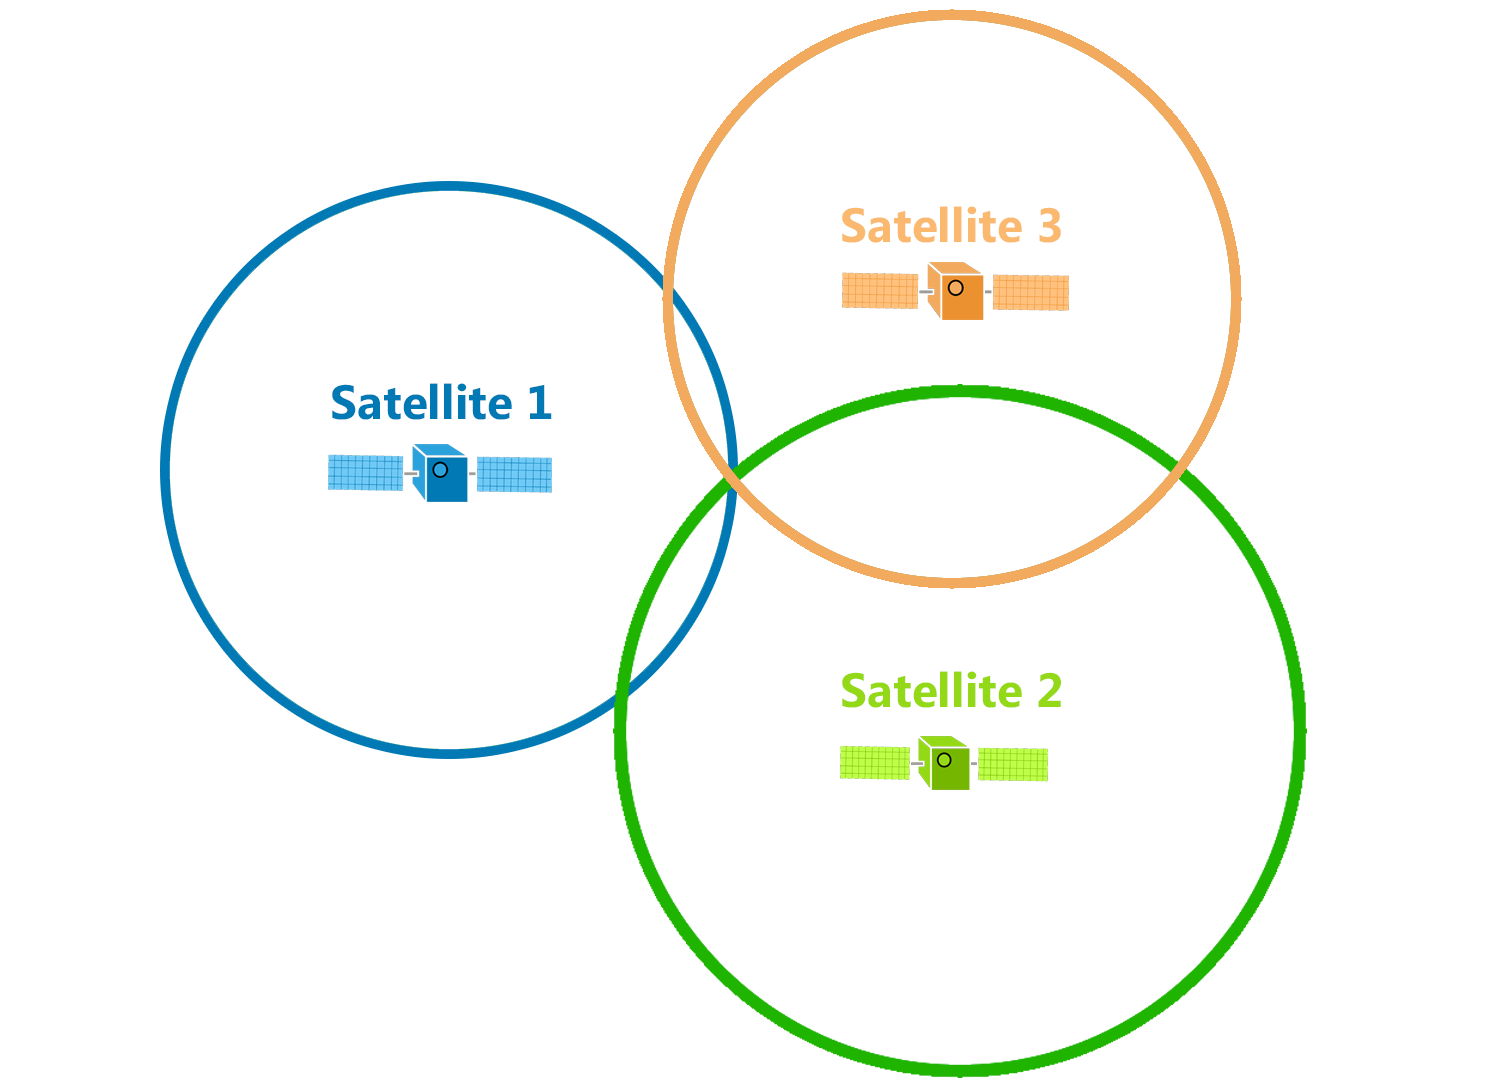
\includegraphics[width=0.48\textwidth]{img/trilateration_2d}
		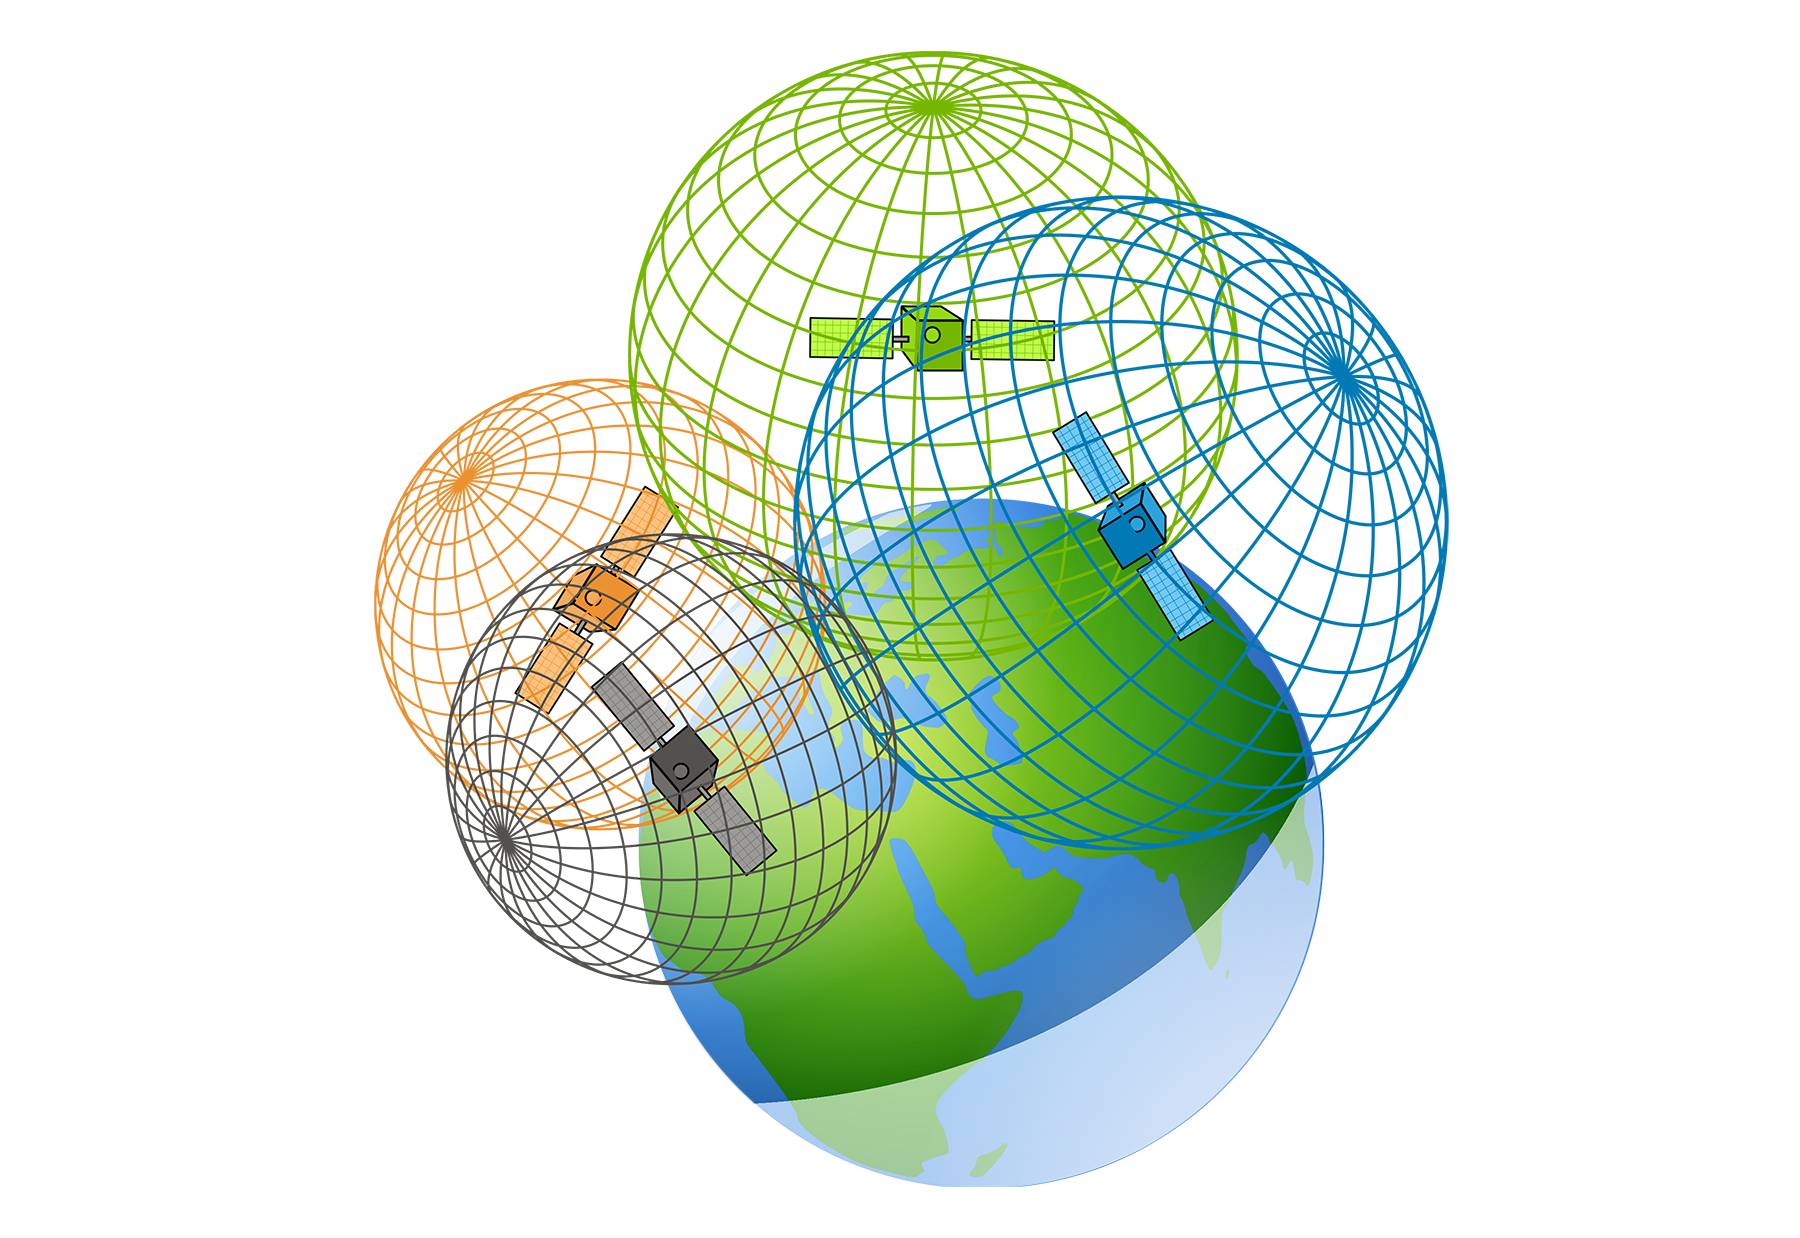
\includegraphics[width=0.48\textwidth]{img/trilateration_3d}
		\par\end{centering}
	\caption{2D and 3D Trilateration (source: \cite{TvTHGPSRW})\label{fig:2d_and_3d_trilateration}}
	\label{fig01c02}
\end{figure}

\textbf{Trilateration} uses distance measurements from at least three devices in particular as \enquote{tri} in the name suggests \cite{RAinWILTaS}. \fref{fig01c02} illustrates usage of Trilateration in 2D and 3D environment. While working in 2D plane will result with only one specific location point. Moving to the 3D plane can create a problem because signal is send in a sphere which could result in more than one position. That is the reason why some systems use at least four signal sources, example of such system is GPS \cite{GNSSGPS}. Advantage is easy implementation and simple calculations. One down side of this approach is that all devices must have synchronized clock \cite{RAinWILTaS}.

\medskip

\textbf{Multilateration} also known as hyperbolic positioning is using Time Difference of Arrival (TDoA) instead of Time Of Arrival (ToA) used in previous case. This approach involves the intersections of hyperbolas rather than circles as shown in \fref{fig02c02}. Main advantage of this method is that only receiving devices must have synchronized clock instead of all \cite{PLTaA}. Multilateration was developed for tracking aircraft position and it is widely used.

\begin{figure}[h!]
	\begin{centering}
		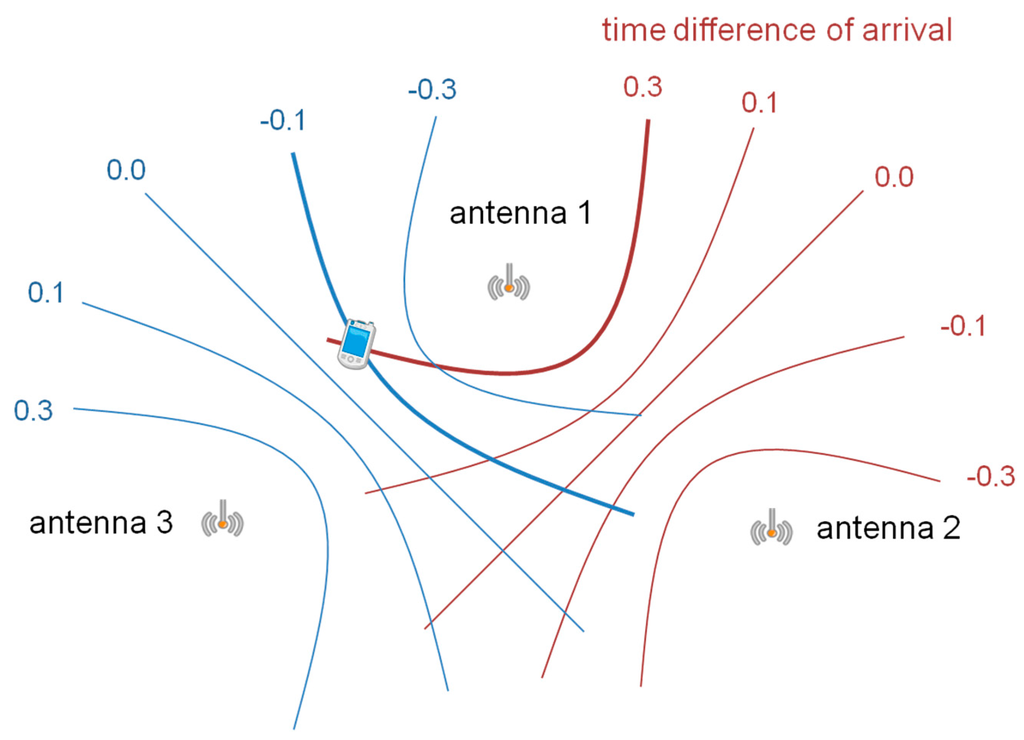
\includegraphics[width=0.6\textwidth]{img/multilateration}
		\par\end{centering}
	\caption{Multilateration (source: \cite{HPwAA})\label{fig:Multilateration}}
	\label{fig02c02}
\end{figure}

Note: At this time term Multilateration is not as strict as it used to be. It can now refer Lateration with more than three devices.

\subsection{Angulation}\label{sec:Angulation}
This technique uses Angle of Arrival (AoA) of radio signals to determine location. It uses highly directional antennas or antenna arrays. Same as Lateration these antennas are placed in known location and basic AoA requires at least two of them to determine position on 2D plane but more of them can be used to improve accuracy \cite{RAinWILTaS}. That makes it an advantage over Trilateration. Second advantage of this approach is no need for synchronization between devices.

There are few disadvantages of this approach since it needs complex hardware setup due to the use of antennas. Other problem is with multipath locations since it can cause signal reflection making it not useful for indoor localization. And final one to mention is the decrease of accuracy when mobile target moves further from the antennas \cite{AoA, RofAoA}.

\begin{figure}[h!]
	\begin{centering}
		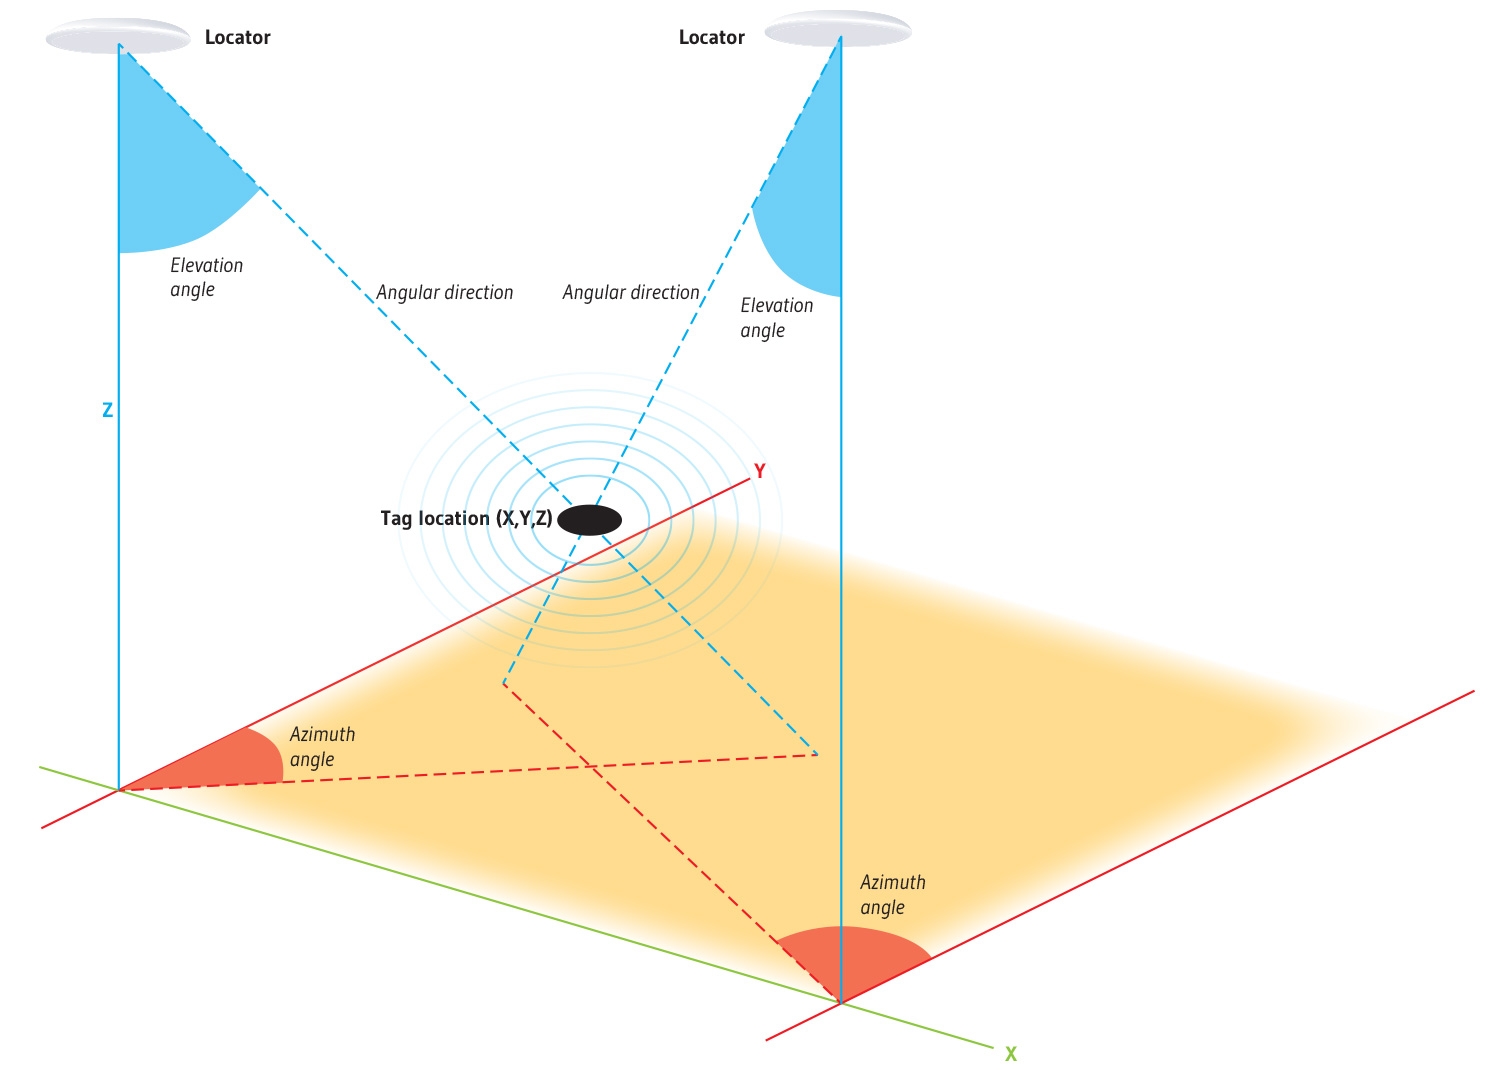
\includegraphics[width=0.6\textwidth]{img/angulation}
		\par\end{centering}
	\caption{3D location using AoA from Quuppa Intelligent Locating System (source: \cite{QAoA})\label{fig:AoAQuuppa}}
	\label{fig03c02}
\end{figure}

\section{Fingerprinting}\label{sec:Fingerprinting}
This method is a part of Signal Strength Fingerprint Maps (SSFM) type. Main point of this approach is using previously recorded data to figure out device location. Hence fingerprint term in the name. There are multiple kinds of radio signal sources such as bluetooth, wireless or cellular devices that can be recorded.

Fingerprinting has two main phases where the first one is fingerprint maps construction also called offline phase. They are created by collecting Received Signal Strength (RSS) and optional extra features in known locations. All these values are saved in the database and it is called fingerprint map. The second phase is localization itself also known as online phase where the device measures RSS values and compares them with fingerprint maps to approximate position using suitable method \cite{LocalizationApproaches, ILWTP}. Most used algorithms or methods to approximate position are \cite{IILUBLEB}

\begin{itemize}
	\item probabilistic methods,
	\item k-Nearest Neighbors,
	\item neural networks,
	\item support vector machine,
	\item smallest M-vertex polygon.
\end{itemize}

There are multiple advantages of this approach and the most important is that it does not need any additional or specialized hardware. Next one is no need for time synchronization between the stations. Both of these advantages make it simple and cost effective method for localization. On the other hand building of the map is very time consuming and needs heavy calibration. It is also susceptible to changes in environment such as people presence, object movement or relative humidity \cite{IILUBLEB, RSSFofIFD}.

\section{Proximity}\label{sec:Proximity}
Proximity detection also known as connectivity based positioning calculates only approximate location. Position is determined by cell of origin (CoO) method with known position and limited range \cite{RAinWILTaS}. Specific device location is based on cell of the connected device (\enquote{associated access} point in Wi-Fi 802.11 systems) as shown in \fref{fig04c02} \cite{WiFiLBS}.

\begin{figure}[h!]
	\begin{centering}
		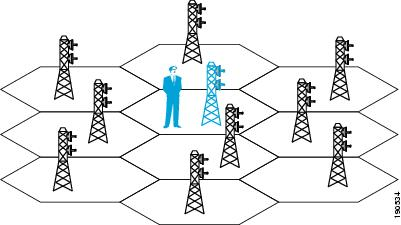
\includegraphics[width=0.6\textwidth]{img/cell_of_origin}
		\par\end{centering}
	\caption{Cell of Origin (source: \cite{WiFiLBS})\label{fig:CellOfOrigin}}
	\label{fig04c02}
\end{figure}

Primary advantage of this approach is very easy implementation and no need for complicated algorithms and thus making calculations fast. However, for various reasons devices can be associated to cells that are not in close physical proximity. Such errors can happen for example in multi-floor buildings where floor cells overlap. There are additional methods that can be used to improve localization such as using received signal strength indication (RSSI), manual method (human search) or connecting to device with highest signal strength \cite{WiFiLBS, RAinWILTaS}.

\section{Other techniques}
\textbf{Scene analysis} is a pattern recognition method that uses features of a scene observed from a particular vantage point to draw conclusions about the location of the observer or of objects in the scene also \cite{LSfUC}. This approach has been used in many applications, such as image and speech recognition, as well as location \cite{LSAWIFI}. The advantage is that the location of objects can be inferred using passive observation and features. The disadvantage is that the observer needs to have access to the features of environment against which it will compare its observed scenes \cite{LSfUC}.

\medskip

\textbf{Dead Reckoning} refers to a position solution that is obtained by measuring or deducing displacements from a known starting point in accordance with motion of the user \cite{DRNS}. Basically calculate new position based on starting point, travel distance and angle of movement. Because new position calculations are dependent on previous ones there is the need for high accuracy of data since it makes errors cumulative \cite{IDRAIP}.
\chapter{Related Work}\label{sec:RelatedWork}
Since this is not a novel idea there are some completed solutions and paper written about Fingerprint collection using multiple devices. This chapter will describe few selected solution close to this one for comparison.

\section{Improving Precision by Using Multiple Wearable Devices}\label{sec:IPUMWD}
Focused on improving indoor localization using BLE-based fingerprinting with multiple devices \cite{IPBLEIUMWD}. Using combination of smart phone and wear should in this case prevent signal obstruction from human body and at least one of the devices should receive beacon signal. Unfortunately due to low BLE sensibility of wear devices, authors decided to supplement them with smartphone, in this case with Nexus 5 running Android 4.4.

This paper proposes calculating medians using 800 millisecond tests where user can move at most one meter. For all medians at the same position is calculated average and variance, based on which a normal distribution is used to model the potential variation of RSSI. One thing to note is that fingerprint maps are built based on facing direction. There are five main scenarios tested

\begin{itemize}
	\item P1: device held in hand where body does not obstruct its LOS path to all beacons,
	\item P2: device is put in breast pocket and LOS may be obstructed to some beacons,
	\item P3: user holds smartphone in hand and wears a smartwatch on one wrist,
	\item P4: one device is put in the breast pocket and the other is on one wrist,
	\item P5: one device is in the breast pocket, and two other devices, each on one wrist.
\end{itemize} 

Firstly, four of these scenarios were tested in a 15x8 meters entrance hall with four deployed beacons in the corners and ten measurement positions. In this location using multiple devices can improve position precision and reduce error by 57\%. \tref{tab1} shows mean errors for previously mentioned cases where using more devices improves localization. However there is one position where case P4 will result with higher error then P3 due to building structure and signal obstruction for nearest beacons.

\begin{table}[h]
	\begin{center}
			\begin{tabular}{| l | c |}
				\hline
				Scenario & Mean error (m) \\ \hline
				P1 & 2.36 \\
				P2 & 1.71 \\
				P3 & 0.96 \\
				P4 & 0.41 \\ \hline
		\end{tabular}
		\caption{Mean errors at first location (sources: \cite{IPBLEIUMWD})}
		\label{tab1}
	\end{center}
\end{table} 

Secondly, all of previously mentioned scenarios were tested in a conference room with unified ceiling and desks near the walls. This location is used to investigate the impact of beacon density to position precision. Three following combinations of beacons are used

\begin{itemize}
	\item A: four beacons at the corners,
	\item B: combination A with one beacon at the center,
	\item C: combination B with four more beacons at the sides of the room.
\end{itemize}

Using directional maps at this location resulted in increase of maximum localization error, which was not expected. This error can increase even more when using higher count of beacons and occurs mostly when testing at the edges of the room. Mean error on the other hand shows an improvement, higher with more beacons used. 

\begin{table}[h]
	\begin{center}
			\begin{tabular}{ | l | c c c | }
				\hline
				 & \multicolumn{3}{ c | }{Mean error (m)} \\ \hline
				Scenario & A & B & C \\ \hline
				P1 & 2.05 & 2.05 & 1.76 \\ 
				P2 & 1.84 & 1.49 & 0.90 \\ 
				P3 & 1.36 & 1.09 & 0.63 \\ 
				P4 & 1.24 & 0.78 & 0.23 \\ 
				P5 & 0.80 & 0.39 & 0.07 \\ \hline
		\end{tabular}
		\caption{Mean errors at second location (sources: \cite{IPBLEIUMWD})}
		\label{tab2}
	\end{center}
\end{table} 

In summary, position error can be improved by three aspects: using more devices, using directional map or increasing the number of beacons. There are two main conclusions of this paper. First, confirmed precision degradation when testing near the edge of the room with obstructed signal from nearest beacon. Second, human body does not greatly change radio signal and device can receive reflected signals with sufficient strength. 

\section{SmartFix}\label{sec:SmartFix}
An Indoor Locating Optimization Algorithm for Energy-Constrained Wearable Devices called SmartFix \cite{SmartFix}. The main goal of this paper is improve energy consumption efficiency for wearable-based indoor localization using WiFi fingerprints. Single real-time experiment of energy consumption was run and split into two main parts: computation of location and collection of fingerprints. According to this experiment, energy consumption caused by collection is occupies 99\% of localization algorithm.

This paper proposes novel indoor localization strategy, SmartFix, that can cooperate with existing indoor localization technologies based on WiFi. It enhances accuracy of such algorithm with a little extra energy cost of calculation but a large save of signal collection energy cost. Aided with machine-learning algorithm, it obtains the relative features given the trajectories of users in certain areas and modify the localization results. SmartFix can save up to 70\% of energy while achieving the same localization accuracy when compared to the original fingerprint method.

To test this new system it was implemented with prototypes of TinyLoc \cite{TinyLoc}, MoLoc \cite{MoLoc} and basic WiFi fingerprint method using k-neighbor algorithm. TinyLoc is more focused on energy efficiency than location accuracy. In contrast SmartFix analyses the history trajectory of people in given area to improve locating results. It refers to user motion features, SmartFix modifies locating results to achieve satisfying accuracy. MoLoc also leverages user motion by collecting trajectory patterns using device built-in sensors.

All previously mentioned prototypes were deployed with and without SmartFix to test its power consumptions. It only needs single real-time RSS signal in the
locating phase to guarantee excellent energy saving performance. \fref{fig6} shows energy consumption of on-time locating on two specific devices: HTC one and Moto 360. 

\begin{figure}[H]
	\begin{centering}
		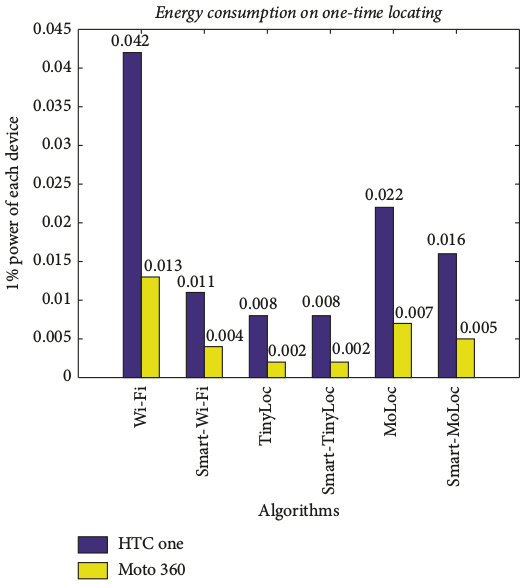
\includegraphics[width=0.6\textwidth]{img/smart_fix}
		\par\end{centering}
	\caption{Energy consumption based on prototypes (source: \cite{SmartFix})\label{fig:SmartFix}}
	\label{fig6}
\end{figure}

This paper proposed an tested new localization technology, SmartFix, which main focus is to improve energy efficiency for wearable devices. According to experiment, the probability of error within 2 meter can be reached in 80\% of cases. Meanwhile, energy consumption is 35\% lower than that of MoLoc with the same accuracy, and SmartFix obtains best accuracy with minimal energy cost.

\section{SmartWatch vs. SmartPhone}\label{sec:SWvsSP}
A comparative study about localization using smartwatch vs. smartphone \cite{SWvsSP}. It presents that positioning accuracy using WiFi based fingerprint implemented on a smartwatch is sufficient for at least room-size locations. Average minimum room size is 10$m^2$ or at least 3 $x$ 3$m$ with maximum of five WiFi APs broadcasting on different channels.

Field study was conducted in six specific locations such as farm, large room, house, two types of medium rooms and one small room. This study collected data using two Android based devices, MotoACTV was used as smartwatch and Samsung Galaxy S3 mini as smartphone. To make fingerprint data more reliable the study collects device orientation (horizontal, vertical) and samples were taken in all four cardinal directions (north, east, south, west).

\begin{figure}[H]
	\begin{centering}
		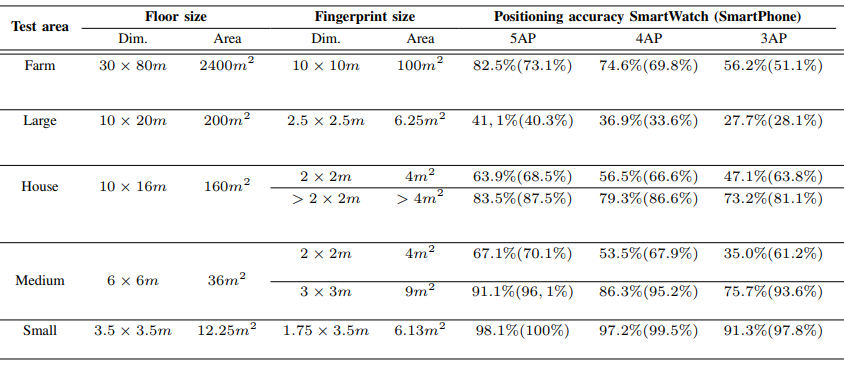
\includegraphics[width=0.9\textwidth]{img/smartwatch_vs_smartphone}
		\par\end{centering}
	\caption{Summary table of results (source: \cite{SWvsSP})\label{fig:SWvsSP}}
	\label{fig8}
\end{figure}

\fref{fig8} shows summary results of experiments. Most important part of this data is comparison of positioning accuracy between smartwatch and smartphone. In all tests the difference in classification error between the smartphone and smartwatch was at most 5\% if data from all five APs is used. On the other hand it can be 25\% worse when using small amount of APs in large environments. The result of this study is a confirmation that localization using smartwatch is comparable to smartphone and sometimes even better for home environments. The usage of smartwatches is also preferable since it is tightly connected to a penson.

\chapter{Android}\label{sec:Android}
This chapter will provide information about Android and WearOS technology from the same company. Why it was developed and what are the differences between previous versions and other wear technologies.

\medskip

Android is a Linux based operating system for mobile and wear devices developed by Google. The main selling point of this system is being an open-source project, meaning everyone can access the code and modify it as they wish. Android was mainly developed for mobile platform but in time moved beyond and can be implemented into all kinds devices, such as wear, tablets, televisions and even refrigerators or cameras \cite{WIGA}.

\section{Android system structure}\label{sec:AndroidSystemStructure}
Android is created as a stack, meaning there are functional modules \enquote{stacked} on top of each other from Linux core over native libraries to applications as shown in \fref{fig01c04}. Android maintains all implementations with complete software stacks to enable device creators to run and modify Android for their specific hardware. To support these modifications and testing every release has multiple \enquote{code lines} to separate stable versions from experimental work \cite{AOSP}.

\begin{figure}[H]
	\begin{centering}
		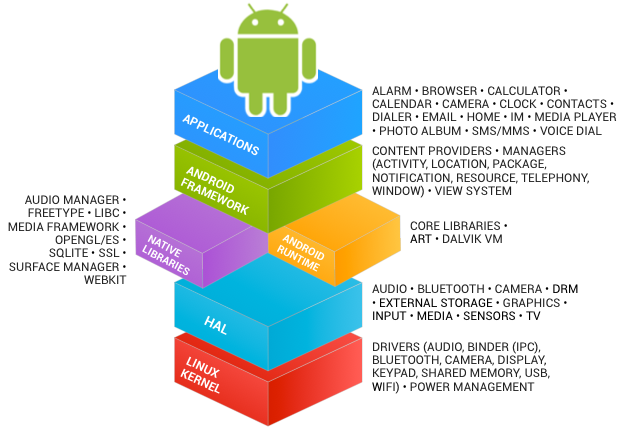
\includegraphics[width=0.6\textwidth]{img/android_stack}
		\par\end{centering}
	\caption{Android stack (source: \cite{AOSP})\label{fig:AndroidStack}}
	\label{fig01c04}
\end{figure}

There are multiple versions of Android system at this time and every single one has its own version information, code name and API level. Version codes are number identifications of a specific system build. Highest levels of these numbers are grouped into code names that are ordered alphabetically. For example, versions 8.0.0 and 8.1.0 have both the same code name called Oreo. Finally API level is number identification for compatibility of specific application and is always compared to API level of device Android system \cite{AOSP, AD}. Devices with API levels lower than minimum level supported by application are not able to run it.

The highest part of the Android system stack are applications which extend device functionality and are written primarily in Java or new Kotlin programming language \cite{SoASTaD}. These application are packaged into \verb|.apk| files, which is a zip archive, containing all application files like Java classes, layouts, images and more. One of the very important files is \verb|AndroidManifest.xml|, it contains all meta-data about the application, such as permissions, package name, used components, versions and so on. These application packages can be shared, for a nominal fee, via official Android market called Google Play. At the end of 2017 there were over three and a half million applications available in Google Play Store \cite{SoASTaD, NoAAiGPS, NoAA}.

Application permissions maintain security for the system and users. Android requires that application declares the permissions it needs before it can use certain system data and features. Depending on how sensitive the area is, the system may grant the permission automatically, or it may ask the user to approve the request. Following example shows how to set required application permissions in \verb|AndroidManifest.xml|, Internet is granted automatically but location must be manually approved by device user.

\begin{lstlisting}[caption=Application permission settings]
<uses-permission android:name="android.permission.INTERNET" />
<uses-permission android:name="android.permission.ACCESS_FINE_LOCATION" />
\end{lstlisting}

Android is platform designed to be open-source and free which also makes it easy to create malicious applications. These application can bypass existing security and steal sensitive data, use telephone services or even gain control over the device \cite{ASIMPD}. Android has multiple ways to protect against such applications one of the most notable ones are Android Permission Framework and Google Play Protect \cite{SoASTaD}.

\section{Wear technologies}\label{sec:WearTechnologies}
Interactive wearable, as an example smartwatches, is a new part of mobile computers. Wear devices are categorically different from mobiles or tables in terms of usage, design and user interfaces (UI). According to the application design guidelines from major vendors users interact with wearable devices frequently throughout daily use. Each interaction is short, often less than 10 seconds, and is dedicated to simple tasks \cite{UtCoAWO}. 

Important thing to note is that there are multiple kinds of wear devices from watches, wristbands, cameras or even glasses \cite{MIWD}. Based on report from Gartner technology research, conducted in 2017, most used wear devices were Bluetooth headsets, wristbands and smartwatches, in this order \cite{GSWWDS}. Thanks to their small size wear devices are ideal to use for hands-free communication and health monitoring.

One problem of these devices is their diversity in hardware and more importantly in software compatibility. Every device manufacturer can create their own operating system for specific wear device and it can be difficult to develop custom applications for it. To avoid such problems this thesis is focused only on smartwatch with WearOS operating system which is based on Android. 

There are three main points to mention considering watch devices. First, small battery capacity that can be almost ten times smaller than of typical smartphone. Second, display size with around forty-times less pixels which completely changes its properties. Finally, scaled down CPU with high efficiency \cite{UtCoAWO}. Last two points are main parts of lowering power consumption of smartwatches but even with these cuts high-end watch devices can have really small battery life only in matter of few days or even hours.

\subsection{WearOS by Google}\label{sec:WearOS}
WearOS by Google, formally known and Android Wear 2.0, is a version of Android operational system tailored to small-screen wearable devices. There are not too many in-system changes from smartphone but one of the main differences can be seen in UI since system had to be adjusted for watch size \cite{CSUITW}. Due to scaled down processing power of watches can offload data wirelessly to mobile for heavy computing tasks, e.g. voice recognition \cite{UCAW}.

\begin{figure}[H]
	\begin{centering}
		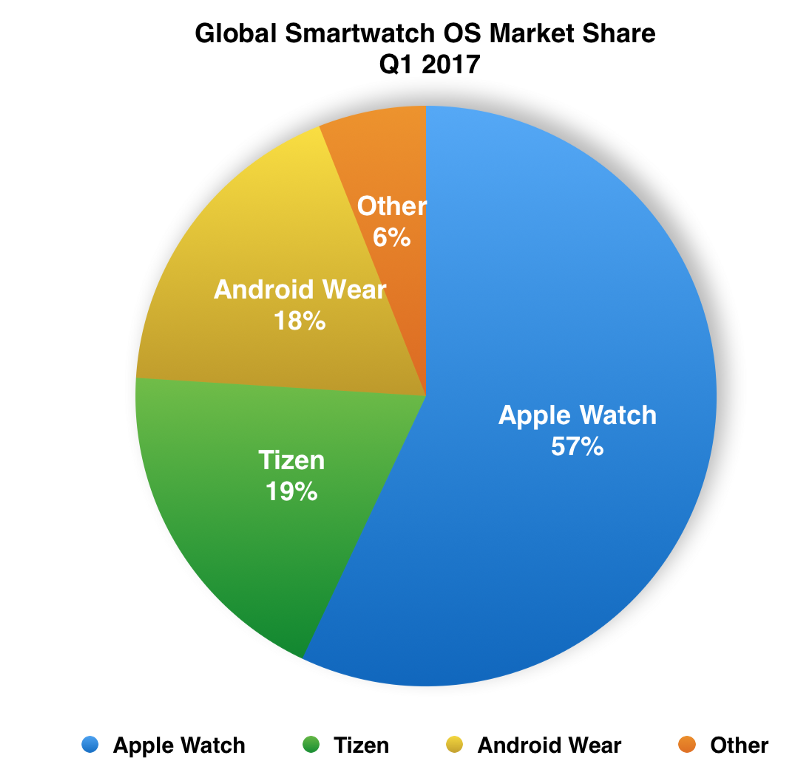
\includegraphics[width=0.6\textwidth]{img/wear_market_share}
		\par\end{centering}
	\caption{Smartwatch OS market share (source: \cite{TOAW})\label{fig:SmartwatchOSMarketShare}}
	\label{fig02c04}
\end{figure}

WearOS is one of the three most popular smartwatch systems but it comes with its own set of problems. Most notable and annoying one is being unable to pair wear with specific mobile device. It can be caused by multiple reasons, such as system compatibility, custom hardware or mobile type and it is more common then it should be \cite{AWPaS}. Having smartphone connected to WearOS can also cause faster battery drain on mobile device. Important thing to mention is that smartwatch can be connected to only single device and connecting to another requires a factory reset. Some other problems can be: software update issues, notifications not coming through to the watch, not being able to connect to WiFi, system crashes and more \cite{WAWP}.

Even with all these problems it is popular system and in early 2017 it got its biggest update yet. New version 2.0, later renamed to WearOS, brought numerous improvements and features where few of the most notable ones will be described in this section \cite{AW2UG, AW2WN, AW2N}.

\subsubsection{Standalone applications}\label{sec:StandaloneApplications}
This feature is crucial change and enables smartwatch applications to run without the need for mobile device to be connected. Before this version it was needed to have smartphone connected to Android Wear when application was supposed to be used. It also supported only connection to Android device and that proved as an obstacle for users without one since they could not use any applications on the watch \cite{AW2UG, AW2WN}.

This change made applications work without mobile and also created the need for them to be installed directly on wear without the need for smartphone. Thankfully part of this update is also standalone Google Play Store where users can browse applications that are designed specifically for the smartwatch \cite{AW2WN}. Part of this feature is also enabling watch to use wireless and cellular networks on their own since most standalone applications require WiFi connection. Finally, as of this update security for communicating between wear and mobile was reworked and improved. Communication is now done via Wearable Data Layer API that is used in almost all Google applications and it is also easy to use for a developer \cite{AW2UG}. 

\subsubsection{UI improvements}\label{sec:UIImprovements}
Part of new Android Wear version is implementation of Android's Material design guidelines \cite{DoAW}. It has much more \enquote{mature} look and darker design for reducing battery drain \cite{AW2WN}. It is completely focused on wear devices and supports both round and square screens with new re-design of application launcher \cite{AW2UG}.

\begin{figure}[H]
	\begin{centering}
		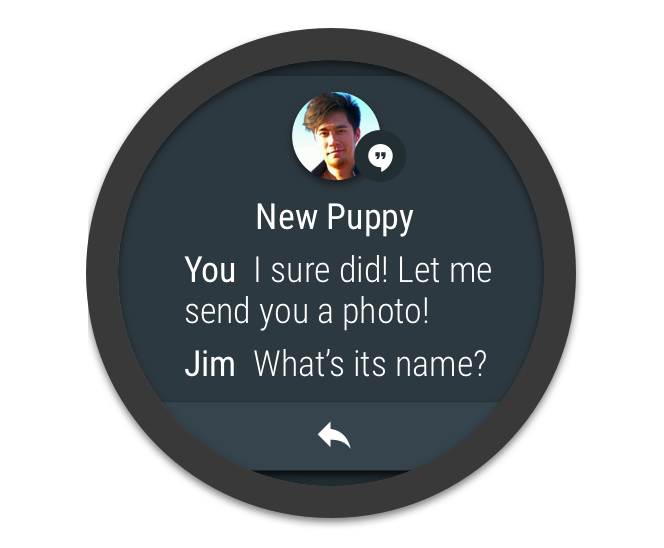
\includegraphics[width=0.3\textwidth]{img/wear_design_notification}
		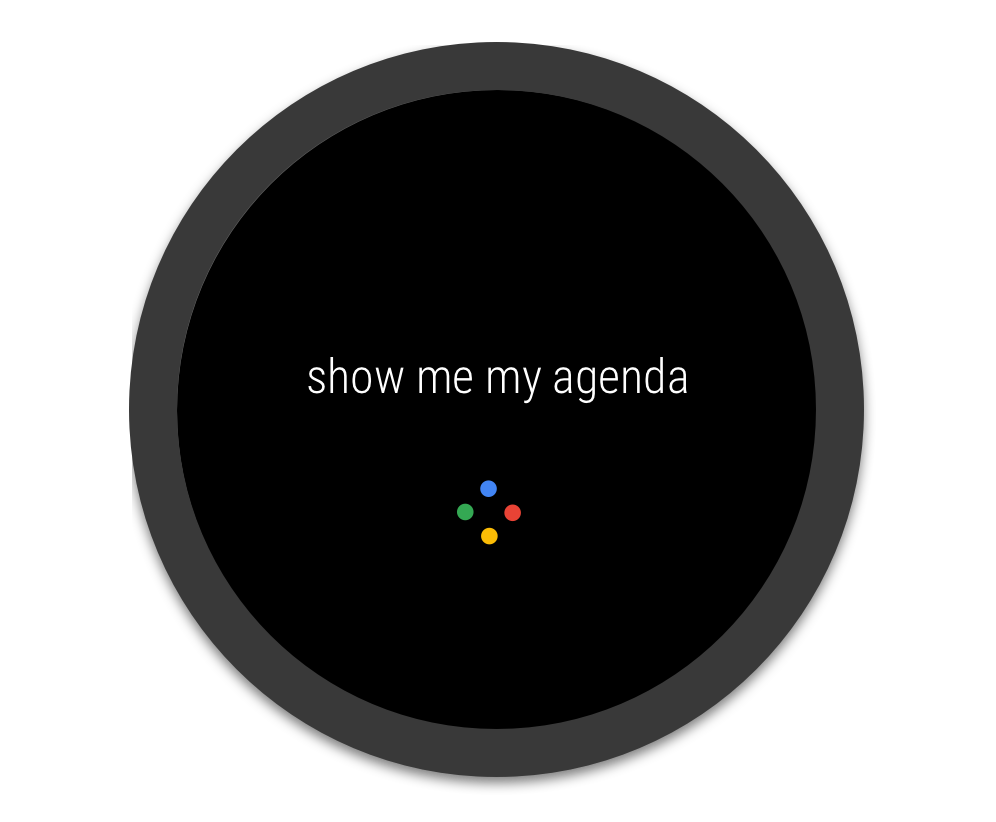
\includegraphics[width=0.3\textwidth]{img/wear_design_agenda}
		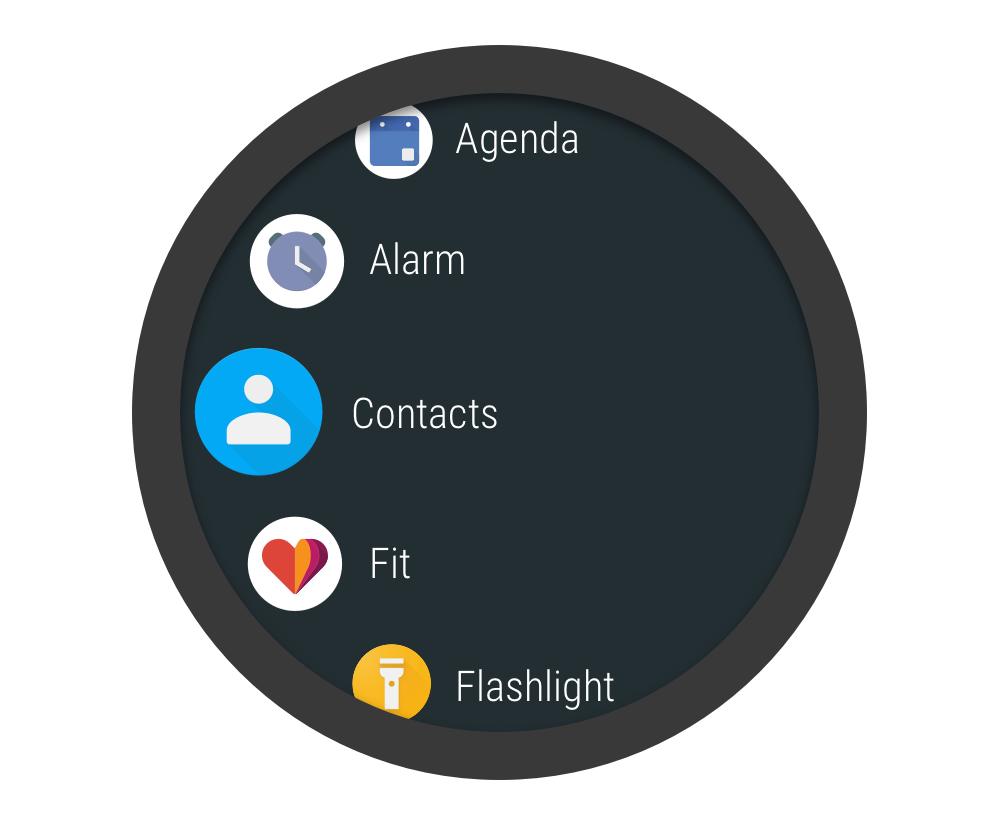
\includegraphics[width=0.3\textwidth]{img/wear_design_menu}
		\par\end{centering}
	\caption{Wear design examples (source: \cite{DoAW})\label{fig:WearDesignExamples}}
	\label{fig03c04}
\end{figure}

Android is also trying to catch up with Apple's watchOS and remade default watch display, also called watch faces, much more useful. Users can add different widgets with data from any application to the watch faces \cite{AW2UG}. This ensures quick access to the information user deems important \cite{AW2N}. All this data displays also match design of currently selected watch face and after clicking it will direct right into the application \cite{AW2WN}.

\begin{figure}[H]
	\begin{centering}
		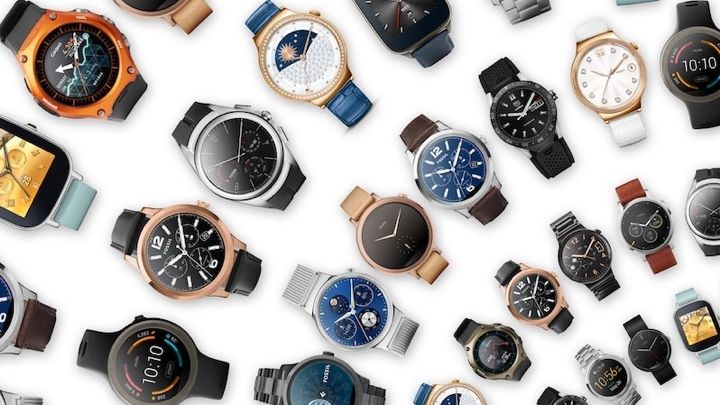
\includegraphics[width=0.5\textwidth]{img/wear_watch_faces}
		\par\end{centering}
	\caption{Wear watch faces (source: \cite{AW2UG})\label{fig:WearWatchFaces}}
	\label{fig04c04}
\end{figure}

\subsubsection{Google Assistant}\label{sec:GoogleAssistant}
Google Assistant is basically voice controlled smart assistant same as, for example, Amazon's Alexa, Apple's Siri or Microsoft's Cortana. There are multiple tech sites that run benchmarks of these systems \cite{ASGA, VACCGASAB, CAGACS, GASBAC} and they do not seem to be that different so there is no need to buy one over the other. These systems can pull information that user needs or wants and they track places of work, sports and daily information, such as schedule, data related to health, interests of the user and much more \cite{WIGA}. With the update of WearOS this assistant is now also available on smartwatches \cite{AW2UG, AW2WN}.

\section{Other wear technologies}\label{sec:OtherWearTechnologies}
During the first years of smartmatches big amount of manufacturers created their own operational systems and flooded the market with them but that was a long time ago and situation changed. Now there are only three main competitors as shown in the \fref{fig02c04} and those are Android (WearOS), Samsung (Tizen) and Apple (WatchOS). Android system was already introduced so it is time for Tizen and WatchOS.

\subsection{Tizen}\label{sec:Tizen}
Between year 2010 and 2012 there were multiple companies developing different wear systems like MeeGo by Nokia and Intel, Samsung Linux Platform (SLP) or Bada created by Samsung. Intel later decided to join forces with Samsung and they created Tizen organization and project which was based on SLP. This project either canceled support of previous systems or merged with them \cite{TOSBHR}. Some of the current members of Tizen organization are: Samsung, Intel, Huawei, Vodafone or SK Telecom \cite{TizenM}.

Tizen system is built from the ground up on Linux platform and is a part of Linux Foundation. It is focused on the needs of all stakeholders of the mobile and connected device ecosystem based on the hardware on which it should run, such as mobile, tv and wearable. One the main focuses of this system is easy support for different manufacturers using easily changeable profiles to suit the needs of a specific manufacturer. Tizen also offers the power of native code development with the flexibility of unparalleled HTML5 support \cite{TizenAbout}.

\begin{figure}[H]
	\begin{centering}
		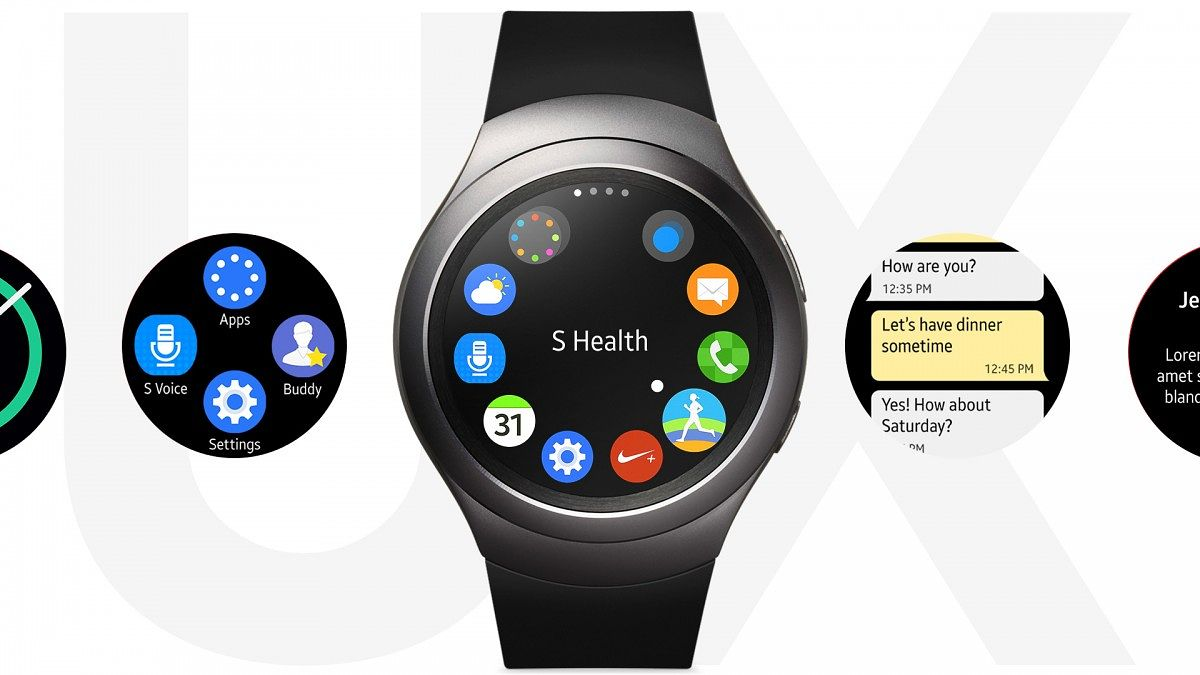
\includegraphics[width=0.6\textwidth]{img/tizen}
		\par\end{centering}
	\caption{Tizen showcase (source: \cite{NFFAWSW})\label{fig:Tizen}}
	\label{fig05c04}
\end{figure}

Developing application for this system can be done in a custom made program Tizen Studio which supports developing native or Web applications where native apps are developed using the C programming language, but since Tizen version 4.0 application can also be developed using .NET or Xamarin UI. This studio contains all required part for developing an application from project management, writing and editing code, debugging and running the application. Newest version of Tizen Studio is 2.3 with the support of Windows, Ubuntu and macOS where the next version will remove support for 32-bit Windows and Ubuntu. Created applications can be deployed to Taizen store which is very similar to Google Play \cite{TizenDev}.

Even though wear version of Tizen OS is deployed only on Samsung products it overtook Android Wear in market shares in the beginning of 2017 but that might change with the release of Wear 2.0 (WearOS). 

\subsection{WatchOS}\label{sec:WatchOS}
Apple started working on smartwatches around year 2002 inspired by sportswatches from Nike with actual results few years later, in 2014, when Apple Watch was revealed to be released in 2015. The release of this smatwatches introduced new version of iOS just for wear devices called system watchOS. Compared to previously mentioned systems this one is the youngest but most popular of them \cite{ATOHAWWC}. WatchOS is currently developed and deployed only for Apple Watches, same as Tizen for Samsung, making Google's WearOS only of them to be implemented by multiple wear manufacturers. First version of watchOS was based on the same principle as Android Wear because it required mobile device to use its applications and luckily for Apple they quickly moved from this interaction in version 2.0. Next versions brought many improvements, such as running application in the background, improved design and support of completely mobile independent application in the newest major version 4.0 \cite{WOS9To5MAC}.

Applications of this system consist of two related bundles: Watch app and WatchKit extension. The Watch app bundle contains the storyboards and resource files associated with application's user interfaces. The WatchKit extension bundle lives inside the Watch app and contains the code for managing those interfaces and for responding to user interactions \cite{AppleDev}.

\begin{figure}[H]
	\begin{centering}
		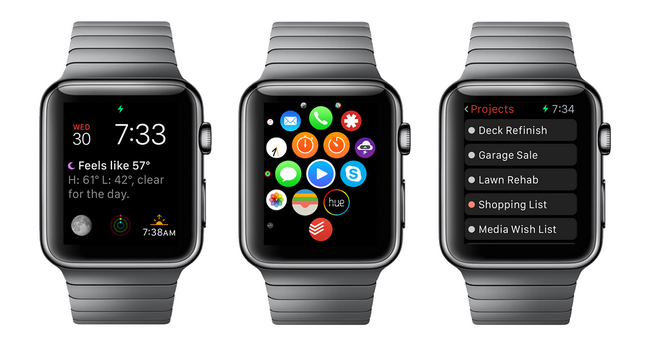
\includegraphics[width=0.6\textwidth]{img/apple_watchOs}
		\par\end{centering}
	\caption{WatchOS showcase (source: \cite{HTFAIAAW})\label{fig:WatchOS}}
	\label{fig06c04}
\end{figure}

Application development for WatchOS can be done using Xcode which is a free program to develop applications for iOS platform created by Apple. Main programming language used in this program is Swift, also created by Apple and based on C and Object-C language. Swift is an open-source language focused on being easy to understand but still powerful and fast. Same as previous wear systems, created applications can be deployed using an App Store similar to Google Play or Tizen store.
\chapter{Application design and implementation}\label{sec:ApplicationDesingAndImplementation}
This chapter describes all important information about created application. First, description of hardware devices used for developing this application. Second, server used to store data on. Third, software libraries used in the application. And finally, implementation of core parts with description of selected code examples.

\begin{figure}[H]
	\begin{centering}
		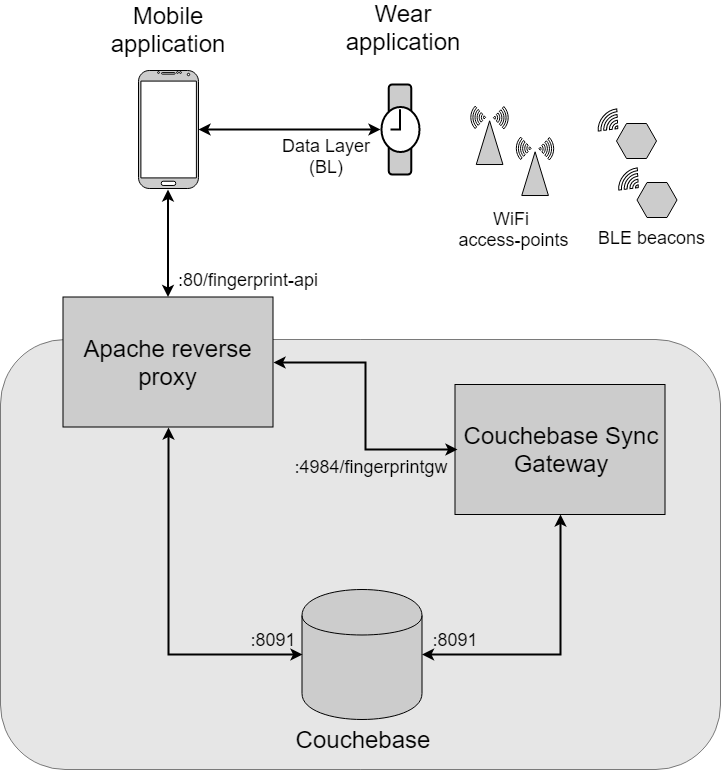
\includegraphics[width=0.6\textwidth]{img/server_architecture}
		\par\end{centering}
	\caption{Application architecture (based on \cite{IILUBLEB})}
	\label{fig01c05}
\end{figure}

\fref{fig01c05} shows core devices and technologies used in this application. There are three main devices of this implementation, mobile, wear and the server. Mobile and wear parts implement scanning for radio signals and they are written in Java language for Android system. Server is also programmed in Java to keep implementations close to each other and make future adjustments easier.

\section{Hardware}\label{sec:Hardware}
There are multiple kinds of hardware devices used in this application. All of them can be seen on previous \fref{fig01c05}, where first and the most important are smartphone and smartwatch. These devices scan for radio signals from WiFi access-points and BLE beacons that are placed in the indoor environment. Final hardware part is the server containing scanned data from all devices and supporting synchronization between them.

\subsection{Smartphone and Smartwatch}\label{subsec:SmartphoneAndSmartWatch}
Both smart devices must support scanning of Bluetooth Low Energy (BLE), which is supported from Bluetooth 4.0, and WiFi signals. Secondary requirements are GSM and LTE modules to support more data types than BLE and WiFi.

\subsubsection{Smartphone}\label{subsubsec:Smartphone}
Main part of the application is developed and tested on Redmi Note 4 from Chinese company Xiaomi. It is running customized version of Android 6.0 called MIUI. Even thought system was customized, in core it is still Android so there are no problems in that regard \cite{XRN4LTE}. This phone has Bluetooth 4.1 with LE support and WiFi 802.11 a/b/g/n chip, thus main requirements for the hardware are met. Concerning secondary requirements, all them are also met with GSM and LTE support like most modern smartphones do \cite{XRN4FPS}.

One interesting thing about Xioami smartphones is their locked bootloader. It prevents users from any manual updates but most importantly from reseting the device to factory settings. For unlocking bootloader owner has to create an account on Xiaomi website and put a request to unlock it, which is usually processed within two weeks period and there is no actual guarantee of it being approved. After evaluation process is complete user will be notified via sms about the result of such request.

\subsubsection{Smartwatch}\label{subsubsec:Smartwatch}
Before development for wear device could begin it was required to find suitable smartwatches running Android Wear 2.0 system. This iteration was quite new at the time, which made it harder to select such device because there were not so many options to choose from. During selection process there were around twenty smartwatches with this system and only five of them were selected for a closer inspection based on few technical articles \cite{BAWW, BAWW18, BAWW17}.

\begin{table}[h]
	\scriptsize
	\begin{center}
		\begin{tabular}{| m{3cm} | c | c | l |}
			\hline
			Watch & BLE / Wi-Fi & Czech Republic & Problems \\ \hline
			LG W280 Sport & Yes / Yes & No & \begin{tabular}[c]{@{}l@{}} Battery life is one day or less. \\ Too big in size. \end{tabular} \\ \hline
			LG W270 Titanium Style & Yes / Yes & Yes & Battery life is one day or less. \\ \hline
			Huawei Watch 2 & Yes / Yes & Yes & \begin{tabular}[c]{@{}l@{}} First update can take a long time. \\ Slight Bluetooth pairing issues. \end{tabular} \\ \hline
			Polar M600 & Yes / Yes & Yes & \begin{tabular}[c]{@{}l@{}} Polar support complains. \\ Phone synchronization issues. \\ GPS location malfunctions. \end{tabular} \\ \hline
			ASUS ZenWatch 3 & Yes / Yes & No &  \begin{tabular}[c]{@{}l@{}} Strap breaks fast. \\ AW 2.0 update can break the watch. \\ ASUS support complains. \end{tabular} \\ \hline
		\end{tabular}
		\caption{Smartwatch comparison (sources: \cite{LGWSP, LGWST, HW2, PM600, AZW3})}
		\label{tab2}
	\end{center}
\end{table}

Only one smartwatch could be selected out of the five displayed in \tref{tab2}. Selection was made based on hardware requirements, website articles and customer experience. First, wear device had to support BLE and WiFi, which all of them do. Second, it must have been sold in Czech Republic (CR) because it makes shipping and warranty dealings easier. Only three of five devices were sold in Czech Republic at that time so others were taken out of the consideration. Final decision was made based on extensive research of customer reviews in shopping sites, such as Amazon, CZC, Heureka, Alza, wear official websites \cite{LGWSP, LGWST, HW2, PM600, AZW3} and other tech sites \cite{BAWW, BAWW18, BAWW17}. In the end, selected device was Huawei Watch 2 since requirements were met and there were not too many problems found in reviews.

Initial setup of the wear device was composed of two main parts. First, update wear system which took about one to two hours. Second, setup the watch and copy Google account information into it, this is where some problem were encountered. Copying of accounts from Redmi Note 4 to the watch never completed successfully. To fix this problem another smartphone (Huawei Y5 II) was used to copy the account and as it was already mentioned, only single device can be connected to smartwatch. Connecting to new smartphone forces a factory reset and removal of all data from wear device. Luckily, there is a workaround for this issue handled via Android Debug Bridge by following this \cite{HtPAWW} article. In short it resets the information about connected mobile device and starts new bluetooth connection search.

Since Google wants to focus also on iOS device technology, Android Wear 2.0 was rebranded to WearOs by Google to remove confusion in the future \cite{AWITFNM}. This forced an update on wear devices, updating it to the newest Android version which resulted in some changes during development process. First, was an implementation bug in scanning library that was introduced and had to be fixed. Second and bigger problem was the inability to deploy new version of the application from Android Studio to the watch. This, for some reason, effected the main computer used to develop this application and it was fixed by using another one.

\subsection{Radio signal devices}\label{subsec:RSD}
Hardware devices used to send out radio signals are BLE beacons, WiFi access-points and Cellular towers. Only first two types of these devices can be placed inside of the building and are most commonly used for indoor localization. Signal from cellular towers is only a complimentary information that does not have to be used and cannot be influenced since they are placed outside by telecommunication companies.

\subsubsection{BLE beacons}\label{subsec:BLEBeacons}
Beacons are small devices that can be easily placed in almost any environment. Only thing they do is send an information packets using bluetooth and nothing else. They are commonly used in museums, airports and as of late for indoor localization \cite{10TABB}. Beacons have their own battery powering them which can last around a year or two without charging because of the new Bluetooth Low Energy (BLE) standard. This technology drastically reduces power consumption and introduces new configuration options regarding advertising interval and transmitter output power \cite{IPSBOBLE}. More in depth description of this technology and devices was written by Pavel Kriz et al. \cite{IILUBLEB}.

\begin{figure}[H]
	\begin{centering}
		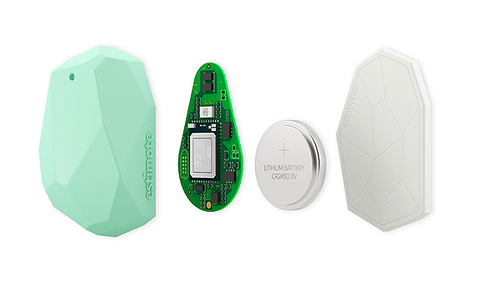
\includegraphics[width=0.6\textwidth]{img/estimote_beacon}
		\par\end{centering}
	\caption{Parts of Estimote beacon (source: \cite{RMPFEB})\label{fig:PartsOfEstimoteBeacon}}
	\label{fig02c05}
\end{figure}

There are multiple beacon manufacturers, each with their own quality, signal strength, battery life and other hardware differences. Changes can also be found in software (packet) specifications for beacons, meaning data they send have different formats but it does not mean other systems cannot see them. Some software changes are usually have to be made to detect different kinds of beacons but they are documented and not hard to make. Beacons are also usually platform independent, making them work with multiple systems, such as Android or iOS \cite{IPSBOBLE, 10TABB}. Beacons used in this thesis are from a company called Estimote and they are most commonly used.

Another important thing to mention, beacons are not connected to the Internet and do not collect any data from devices around them. That is why all data have to be processed in another device, most commonly a smartphone, but it also makes beacon safe to use because there is no need to worry about theft of user sensitive data \cite{10TABB}.

\subsubsection{WiFi access-points}\label{subsec:WiFiAccessPoints}
WiFi signals are most common devices used in indoor localization due to their presence almost anywhere and high precision. In this case, several WiFi transmitters of the \verb|eduroam| network made by Cisco were used. This network allows users (researchers, teachers, students, staff) from participating institutions to securely access the Internet from any eduroam-enabled institution \cite{Eduroam}. Access-points are permanently deployed on every floor of the Campus building and cannot be influenced or have their settings changed, they are also usually at least two per location to enable transmitting in 2.4 GHz and 5 GHz band.

\section{Server}\label{sec:Server}
This application does not necessarily need a server for its core functionality but it is common and faster to run an analysis of collected data and other heavy computational work on a different and usually faster device. Functionality of the server is to provide a backup of the data and also work as a synchronization point to enable other devices to download fingerprints and upload newly collected ones.

The server infrastructure was built in previous years \cite{IILUBLEB} but it was modified for this solution. In its core server uses NoSQL database to save fingerprints. This type of database does not have a fixed scheme, making it easy to save all kinds of data without any constraints. There are many implementations of NoSQL databases, currently over 225, to choose from. Selected database is called Couchbase, it saves data in JSON files with its very own query language similar to SQL. Part of this database can also replicate data between other devices which could be used in the application part but it was deemed too slow and data heavy for use in this application. Not using this feature created the need for development of a middleman API for communication between Android application and Couchbase database.

As \fref{fig01c05} shows server has three main parts to work with. First, already mentioned Couchbase database to keep scanned data. Second, sync gateway that can synchronize data between devices, which is not used in this implementation but there is a connection to it for specific reason described later. As it was mentioned, these two parts were already implemented in previous years \cite{IILUBLEB}. Final part is a newly created web application working as a REST API to send data between the server and mobile application. 

This API is written in Java-based framework called Spring to keep the code similar to Android. Before implementing, it was documented using Swagger and it handles two main HTTP routes: \textbf{fingerprints} and \textbf{fingerprints-meta}. Mobile application checks meta data on the server before any tasks can be run. It is done by calling \textbf{fingerprints-meta} route which returns count of new fingerprints and last time current device saved new ones on the server. With this information the application calculates how many fingerprints to upload and download, both of these task run in parallel to speed up the process. To prevent device memory exhaustion and connection timeouts both of these tasks have specific limits, download can process 100 of fingerprints while upload only 20 per call. Server can also generate data files for analysis, split by technology, time, origin device and other filters. To simplify this generation it is similar to loading of all fingerprints, it does not create file with the data but prints the them directly into the connection stream.

One last thing to note in \fref{fig01c05} is the connection with sync gateway. Even though it is not used in this implementation for synchronization, it is used to save fingerprints into the database. When data is saved into the Couchbase directly, sync gateway will not be able to display them, that is why the upload goes through the gateway. It ensures all previous and next solutions will be able to use this feature without loosing any important data.

\section{Application Software}\label{sec:ApplicationSoftware}
Software part for smartphone and smartwatch is built on Android system which was already described in \hyperref[sec:WearOS]{Chapter 3}. This section will provide basic information about libraries, technologies and systems used in these applications.

\subsection{AltBeacon Library}\label{subsec:AltBeaconLibrary}
Android core does not allow scanning for BLE beacons, that is why this feature must be implemented in a library extending system features. There are multiple solutions that can be used to scan for beacons such as Estimote SDK \cite{ESDKfA} which was already used in previous thesis \cite{PMRIL}. To change things up BLE beacons are scanned using AltBeacon Library \cite{ABL}.

There was no open and inter-operable specification for proximity beacons at the time and Radius Networks decided to create the AltBeacon specification as a proposal to solve this issue. It is an open and free specification for BLE beacons with the focus to create an open and competitive market for implementation of these devices \cite{AltB}. Basic configuration of this library can scan for beacons based on this standard but it also supports Eddystone beacons which is Google's open-source format. To support, already mentioned and used Estimote beacons, this library configuration must be altered to support their detection. Luckily, scanner function can be easily modified to support different kinds of beacons by adding just one line of the code \cite{ABL, EDDF}.

\begin{lstlisting}[caption=Code to enable all beacon types]
beaconManager.getBeaconParsers().add(
	new BeaconParser().setBeaconLayout("m:2-3=0215,i:4-19,
		i:20-21,i:22-23,p:24-24"));
\end{lstlisting}

This library uses publish-subscribe design pattern, meaning one scan data is send to multiple clients if they listen for them. Using this approach has an advantage of eliminating the need to run scan per client. Update to Android 8 introduced a bug in this feature making it unable to confirm the registration of a client so the scanner had to be reworked to work around this bug, thus postponing the data collection and analysis.

\subsection{Database}\label{subsec:Database}
This solution makes use of two different types of databases to store all the fingerprint data for calculations. First, SQLite database implemented in Android mobile application to save fingerprints from smartphone and smartwatch. This database is a default implementation and most commonly used in Android. Second database type is Couchbase, implemented on the server \textbf{beacons.uhk.cz} to keep all fingerprints in one place and also enable synchronization plus data analysis.

\subsubsection{SQLite database}\label{subsec:SQLiteDatabase}
SQL (Structured Query Language) is a standard language for storing, manipulating and retrieving data in databases. It is a type of relational database, meaning all data is saved into tables with specified rows and columns \cite{WISQLITE}. These tables usually have a set amount of rows with specific names that protect from adding wrong data, for example, you cannot add data \verb|Person(name, surname, eye color)| into table \verb|Person(name, surname)| because there is no column named \verb|eye color| in the table.

Structured data is one of the advantages for this database type and it makes calculation faster but as a drawback it uses more storage space. Other advantage is that data can be saved only once and can be connected to each other. It supports complex queries for creating, reading, updating and removing data (CRUD) and better security with user and table management. Some disadvantages of this system can be in complexity and inflexibility of database schema because it is hard to setup and does not allow saving of data not defined in the tables \cite{ERDMS}. Altering schemes in the future can be really complex since there is the need to parse current data into newly created tables which do not need to have the same schema as current ones.

Since SQL with all its features can consume a lot of hardware resources for a smartphone, Android decided to implement lite version of this database. SQLite has the following noticeable features: self-contained, serverless, zero-configuration, transactional \cite{WISQLITE}.

\begin{itemize}
	\item Serverless = does not need second process for the server.
	\item Self-Contained = requires minimal support from operating system.
	\item Zero-configuration = no need for installation or any configuration.
	\item Transactional = data are protected against failed changes (application crashes, power failure, malformed data and more).
\end{itemize}

\subsubsection{Couchbase database}\label{subsec:CouchbaseDatabase}
SQL-based databases can be complex to implement, scale and usually require more data storage space. This created a motivation to develop so called NoSQL databases. Their most important and significant feature is not having a fixed schema, that makes them easy to scale and replicate between multiple devices. There are over 225 NoSQL databases at this time and selected Couchbase is one of them \cite{NOSQLDB}.

Couchbase is distributed, document-based database with its own querying language called N1QL. It is a database focused on simple server configuration and easy usage for clients, with built-in caching layer and distribution system it does not require any changes in the application. There can be either one server instance of Couchbase or multiple connected effectively creating a database cluster which holds all the data in multiple locations (nodes) \cite{GSWCBS}. This data is saved in JSON file format and usually in readable form without any encryption.

\begin{lstlisting}[caption=JSON format example]
[
	{ "id":"1", "name":"Joe", "lastName":"Doe", "address":{} },
	{ "id":"2", "name":"James", "lastName":"Named", "address":{} }
]
\end{lstlisting}

Since SQL language is used for decades and it became the standard for working with data in databases, Couchbase embraces this approach and extends it for JSON files, creating a new language called N1QL. It has all the main features of the SQL with some minor improvements \cite{WINQL}. Currently this language can be used only on the server implementation and it is not supported in Android. Version of this database for mobile application is called Lite and so called \textbf{views} are used instead of N1QL. Views are objects containing selected data from database documents and their major problem is being very data heavy which is shown in the following section. This makes it one of two main reasons why mobile application uses an SQLite instead of Couchbase. Second point is to differentiate between previous solutions and test data consumption and loading speed of SQL database.

\subsubsection{Comparison}\label{subsubsec:Comparison}
Both of previously mentioned database solutions were tested in Android mobile application to figure out which one is faster and takes less data storage space. As a test, 315 fingerprint documents were loaded and displayed, all of them have more than 500 sub-documents which makes about 150 000 documents in total. As shown in the \tref{tab3}, SQLite takes less storage space and is almost three times faster in loading all the documents, that is why it was selected for this project. If Couchbase Lite would have faster query time or supported the use of N1QL it would be a preferable solution but it is not at this time.

\begin{table}[h]
	\begin{center}
		\scriptsize
		\begin{tabular}{| l | c | c |}
			\hline
			Database type & Data size & Loading speed (315 documents) \\ \hline
			SQLite & 15MB & 23 second \\ \hline
			Couchbase without views & 31MB & 65 seconds \\ \hline
			Couchbase with views & 91MB & 65 seconds \\ \hline
		\end{tabular}
		\caption{Couchbase vs SQLite (sources: \cite{LGWSP, LGWST, HW2, PM600, AZW3})}
		\label{tab3}
	\end{center}
\end{table}

Selecting SQL comes with a disadvantage since it does not provide any data synchronization, due to that, a custom solution must have been created which was already described in the \hyperref[sec:Server]{Server} section.

\subsection{TileView}\label{subsec:TileView}
There are multiple ways to display image map in Android, default solutions usually load the whole picture at once. This works for smaller pictures but it does not necessarily work for bigger ones because the application can run out of allocated memory. To solve this problem it is usually better to try external library or widget created specifically for displaying such images. One approach is to use 2D or 3D library to display image, these libraries usually work with the image as a whole and implement complex functionality to display it without memory exhaustion. The other approach, also used by Google Maps, is to cut the big image to smaller parts, called \textbf{tiles}, display them next to each other and recreating overall image. This approach has multiple advantages.

\begin{itemize}
	\item Solves performance issues and enables cartographers to create aesthetically pleasing maps without the need to worry about performance impact.
	\item When user is panning, relevant pictures stay displayed while others are loaded, thus improving user experience.
	\item Every zoom level has its own collection of images, this makes it easy to keep a good image quality for all zoom levels.
	\item When zoomed in, pictures out of the screen do not have to be kept in memory, this cannot be done with other solutions because image is not split into parts.
	\item Zoomed image can have more details than original one.
\end{itemize}

\begin{figure}[H]
	\begin{centering}
		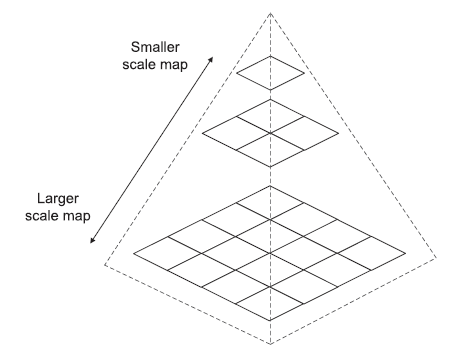
\includegraphics[width=0.6\textwidth]{img/tile_pyramid}
		\par\end{centering}
	\caption{Tile pyramid for zoom levels (source: \cite{WTM})\label{fig:TilePyramid}}
	\label{fig03c05}
\end{figure}

Tiles are images that have 265x265 pixels but that is not the requirement. There is one tile with the image displayed for the lowest zoom, level 0, which is usually not used and level 1 is used instead where each zoom increase splits every tile image into 4 more tiles. For practical purposes, maximum zoom level is usually around 21 with almost 4.5 trillion tiles.

Creating tiles by hand can be really time consuming job, even for low zoom levels, but it can also be done automatically using script or a program. For example, it is possible to create them by slice tool in PhotoShop, but this solution supports only low level of zoom since it has a limit for amount of such created images. Author of this library provides a solution to this problem using a free tool called ImageMagick, which can resize, crop, cut and create images using a command line making it easy to develop a script for all zoom levels required \cite{TileView}.

\begin{lstlisting}[caption=Creating tiles using ImageMagick]
C:\*path to imagemagick*\convert C:\*path to big image*.png 
	-crop 256x256 
	-set filename:tile "%%[fx:page.x/256]_%%[fx:page.y/256]" +repage +adjoin 
	"C:\*path to tile folder*\tile-%%[filename:tile].png"
\end{lstlisting}

This code will split image.png into 256x256 tiles, and name them \enquote{tile-i-j.png}, where \enquote{i} is the column index and \enquote{j} is the row index. More information can be found in the TileView wiki \cite{TileViewWiki}.

\section{Application implementation}\label{sec:ApplicationImplementation}
Implementation of this application is split into two core parts, mobile and wear. Both of them have to implement two tasks in order to be able to create fingerprint maps. First, a scanner for radio signals which will record Bluetooth Low Energy beacons, WiFi access-points and Cellular towers. Second, communication between both implementations, mobile and wear, to allow sending fingerprint data between them. Those are two core functions for both applications but since the synchronization server is used, mobile part also has to communicate with the server.

Both of these applications are programmed in Java language using Android Studio, each of them has a separate configuration and is aimed to different system versions.

\subsection{Scanner}\label{subsec:Scanner}
Scans for radio signal and creates a fingerprint with specific position, device, radio signals and selected sensor information. This additional data, especially about the device, will help with analysis by splitting data into specific groups. There are multiple parts to this task and most of them are very computational heavy so it is better to implement it in a separate \textbf{Thread} to prevent application from freezing. Android provides multiple solutions for running tasks in separate threads.

\begin{itemize}
	\item AsyncTask - simple solution, mainly focused on short running tasks (in seconds). This implementation is easily created since it handles all basic functions like running task, run code before and after task, publish progress to main application thread and many more.
	\item Service - mainly focused on long running tasks which are run immediately after it is started without checking device resources. Android wants to deprecate this approach and develop their new solution, JobScheduler.
	\item Custom thread - one of the hardest solutions to implement because developer has to handle all the tasks related to threads life-cycle and be careful to prevent creation of multiple unwanted threads that might freeze the application or even operating system.
	\item JobScheduler - One of the newest implementations, it is focused to intelligently schedule tasks and run them when the device has required resources ready.
\end{itemize}

Scanner is run using JobScheduler, which is a new technology and Android wants to continue developing this feature. Handling scanned data is implemented using publish-subscribe design pattern handled by \textbf{BroadcastReceiver}. There are two separate receivers, one for Bluetooth Low Energy and second for WiFi data, cellular scanner is connected to WiFi receiver and sensor scanning uses different implementations.

\subsubsection{JobScheduler}\label{subsubsec:JobScheduler}
This feature was introduced in Android 5.0 and it remains under active development with major changes in Android 7.0 version. This platform collects information about jobs that need to run across all the applications. Some of the collected information about specific jobs are: required network access, is the job periodic, should the job be re-scheduled after device restart and many more. This information is used to schedule and run jobs at, or around, the time they were scheduled. JobScheduler is intelligent about running jobs and it uses so called batching, which combines multiple jobs to reduce battery consumption \cite{AD, SOTAJS}.

\begin{lstlisting}[caption=Schedule Firngerprint scanner job.]
// Building job to run
JobInfo.Builder jobBuilder = new JobInfo.Builder(FingerprintScanner.JOB_ID, new ComponentName(getPackageName(), FingerprintScanner.class.getName()));
jobBuilder.setOverrideDeadline(1000);
jobBuilder.setPersisted(false);
jobBuilder.setExtras(bundle);
// Run created job
JobScheduler jobScheduler = (JobScheduler) getSystemService( Context.JOB_SCHEDULER_SERVICE );
jobScheduler.schedule(jobBuilder.build());
\end{lstlisting}

This code is used to schedule fingerprint scanner. Firstly, a job has to be created with specific identification and class to contain job code. Secondly, job information are provided for the scheduler: this task should start around a second after scheduling, it is not run after device restart and there are custom data send to it via \verb|setExtras()| function. Finally, job scheduler is loaded, job constructed and scheduled to run. One thing to remember is to not create a new instance of JobScheduler class because it is a system service.

\subsubsection{BroadcastReceiver}\label{subsubsec:BroadcastReceiver}
Broadcast messages are send from Android system and other Android applications, similar to the publish-subscribe design pattern. This messages are send when an event occurs, such as system boot up, start of device charging cycle or network connectivity change. In addition to system events, custom ones can be created in the application to inform other applications, including itself. When a broadcast is sent, the system automatically routes it to application that have subscribed to receive that particular type of broadcast \cite{AD}. Following code illustrates how easy is to send a custom broadcast identified by specific action, which can be either system or custom. It sends BLE beacon data to be received and parsed into custom beacon entry in the scanner. Last line of the code sends broadcast to be received by other applications.

\begin{lstlisting}[caption=Send broadcast with BLE beacons found.]
Intent intent = new Intent();
intent.setAction(ACTION_BEACONS_FOUND);
intent.putParcelableArrayListExtra(ACTION_BEACONS_DATA, foundBeacons);
sendBroadcast(intent);
\end{lstlisting}

Receiving broadcasts in application has two main steps. First, register the receiver implementation and specific broadcast message it should receive, this can be done via android manifest file or dynamically in the code. If receiver is registered using manifest, application is also launched, only if it is not running already, when the broadcast is sent. Second, create an implementation of BroadcastReceiver class that will handle broadcast information and data using \verb|onReceive()| function.

There are two receivers used in the scanner. First, used for WiFi scanning since it is a default Android solution. Second, BLE scanner was modified to use this approach because there are multiple parts of this application that can scan for surrounding beacons. Other two scanners use \textbf{Listeners} which are interfaces handling communication between system and application.

\subsection{Device communication}\label{subsec:DeviceCommunication}
In this application device communication is used to send fingerprint data between devices using bluetooth. Mobile application sends information about newly created fingerprint such as location and scan duration, these values are the same for both devices. Wear application will, in return, send result data after scan was finished to save it into the mobile database.

First implementation of this feature was build upon bluetooth chat example application from Google. This implementation was using three separate threads to make connection, authorize it and then to send the data when devices were connected. Both of the devices had to accept the connection to send the data, which is normal, but there were some connection loss issues where one of the devices was considered connected and sending data while the second device was disconnected and not receiving anything. That is the main reason why this solution was removed at early stage of the development and substituted with Google's Data Layer API.

To limit power consumption of this application on wear it does not run constantly. Before each scan is started, mobile informs wear to start the application, after startup, confirmation is send back to mobile to initiate sending of fingerprint data. After wear receives the data it starts a new scan for radio signals and later returns the fingerprint back to mobile right after scanning finishes.

\subsubsection{Data Layer API}\label{subsec:DataLayerAPI}
Data Layer is commonly used by Google to send data between their applications. There is an implementation built completely on this feature called Google Tag Manager which sends data from websites to other Google-based tools like Analytics or Adwords. In this case it is a JavaScript object or variable creating virtual \enquote{layer} of the website application which contains various data points, making its name, Data Layer \cite{GTMDL}.

Since it proved as a useful solution it was also implemented for Android and is currently a part of Google Play services. The Data Layer API allows to store and retrieve data between different devices and also kinds of devices, it this case between mobile phone and wear. There are multiple ways to send data depending on what type of data should be sent \cite{AD}.

\begin{itemize}
	\item Data Item - provides a data storage that is synchronized between devices. Whenever data changes, all of the devices using this item are then informed about the change. All data are identified by its own specific Uri containing creator device and path.
	\item Asset - used to send binary blobs of data, such as images. It takes care of the data transfer automatically using caching to avoid sending the same data multiple times.
	\item Message - Good for sending small amounts of data or remote procedure calls, such as controlling mobile media player from wear. If the device receiving data is connected, sender receives a result code confirming successful data send. Although the result code does not guarantee delivery of the message and if the application requires data reliability it should use Data Items. 
	\item Channel - Transfers large data entities, such as music and movie files. It saves the disk space over Data Item or Asset because it does not create a copy of the message on local device before synchronization. It can also be used to transfer streamed data, such as music pulled directly from the network.
\end{itemize}

This application uses message system and data items, where messages are used to send information for wear application to startup and confirm if it was started. Fingerprint data are then send via data items. Since application may be either in the foreground or background there is a need for two solutions to receive the data. First, service that runs when the application is not started or in the background. Second, any activity can implement an interface that will get received data in the foreground.

One important thing to mention is, to send the data successfully between the devices they must have the same APK signatures, meaning they must be signed by the same key. For example, debug versions of two applications developed on two different computers will not be able to send data due to this restriction.

\subsection{Server communication}\label{subsec:ServerCommunication}
Main task of communicating with the server is to synchronize data on the mobile, downloading previous fingerprints and upload newly scanned ones. This feature uses server API to transfer data and since it is a very data and computational heavy, it is implemented in a separate thread, same as a scanner using JobScheduler. It was already mentioned that server API is documented in Swagger, this tool can also generate Android code to communicate with the server, based on defined functions in the documentation. This will generate working code without the requirement of using secondary library but the code is unnecessary complex and so this application uses external library called Retrofit.

Even though the new version of Google's WearOS makes this feature easier to implement on the wear device, it is still used only in the mobile application for one simple reason: to lower power consumption. 

\subsubsection{Retrofit}\label{subsec:Retrofit}
Retrofit is a library turning HTTP API into a Java interface making the implementation easy and simple. This interface contains calls with parameters based on the API documentation, it can return either raw response or automatically convert the data into Java classes based on the configuration. Creating the interface is only one of two parts to make this library working. Second is to create an instance of this library's main class with a configuration specific to the API and use it to initiate calls.

\begin{lstlisting}[caption=Retrofit interface example]
public interface ApiConnection {
	@GET("fingerprints")
	Call<List<Fingerprint>> getFingerprints(@Header("deviceId") String deviceId,
		@Query("timestamp") long timestamp,
		@Query("limit") int limit,
		@Query("offset") long offset);
}
\end{lstlisting}

Previous code contains a small example of Retrofit's interface class with a function for getting fingerprints. First, Retrofit must be informed which type of HTTP call it should use, such as GET, POST, PUT or DELETE. Part of this information can also be URL path added to the call, \textbf{fingerprints} in this case. Secondly, all of the parameters with information where they should be posted, in header, body or query.

\begin{lstlisting}[caption=Retrofit configuration example]
Retrofit retrofit = new Retrofit.Builder()
	.baseUrl("http://beacon.uhk.cz/fingerprint-api/")
	.addConverterFactory(JacksonConverterFactory.create())
	.callbackExecutor(Executors.newSingleThreadExecutor())
	.build();
\end{lstlisting}

There is only one required configuration to make Retrofit working and that is defining the base URL so the library knows where to send the calls. Some other configurations might be adding data converter which converts the data from Json to Java classes, run calls in different threads or create custom HTTP client.

\subsection{Application screens}\label{subsec:ApplicationScreens}
Mobile application has three screens, map and scanner, surrounding devices, synchronization screen and wear application has only one containing information about current scan. All of these screens are made to as simple for use as possible.

\subsubsection{Map and scanner}\label{subsec:MapAndScanner}
This screen is the core of mobile application and it shows the map of a building floor with fingerprint positions as markers. Map is implemented using TileView library previously described in this chapter. It is used to display locations of fingerprints and enable to create new ones, provide data about existing ones and enable to delete them. Deleting was not supposed to be part of this implementation but it proved useful when one or both devices collected \enquote{broken} fingerprints, which are usually created by failure in WiFi scanning or failing of sending data from mobile to wear device. Deleting removes last created fingerprint group at specific spot, meaning it deletes one fingerprint per device type. This is possible because fingerprints have their specific scan id connecting them together.

\begin{figure}[h!]
	\begin{centering}
		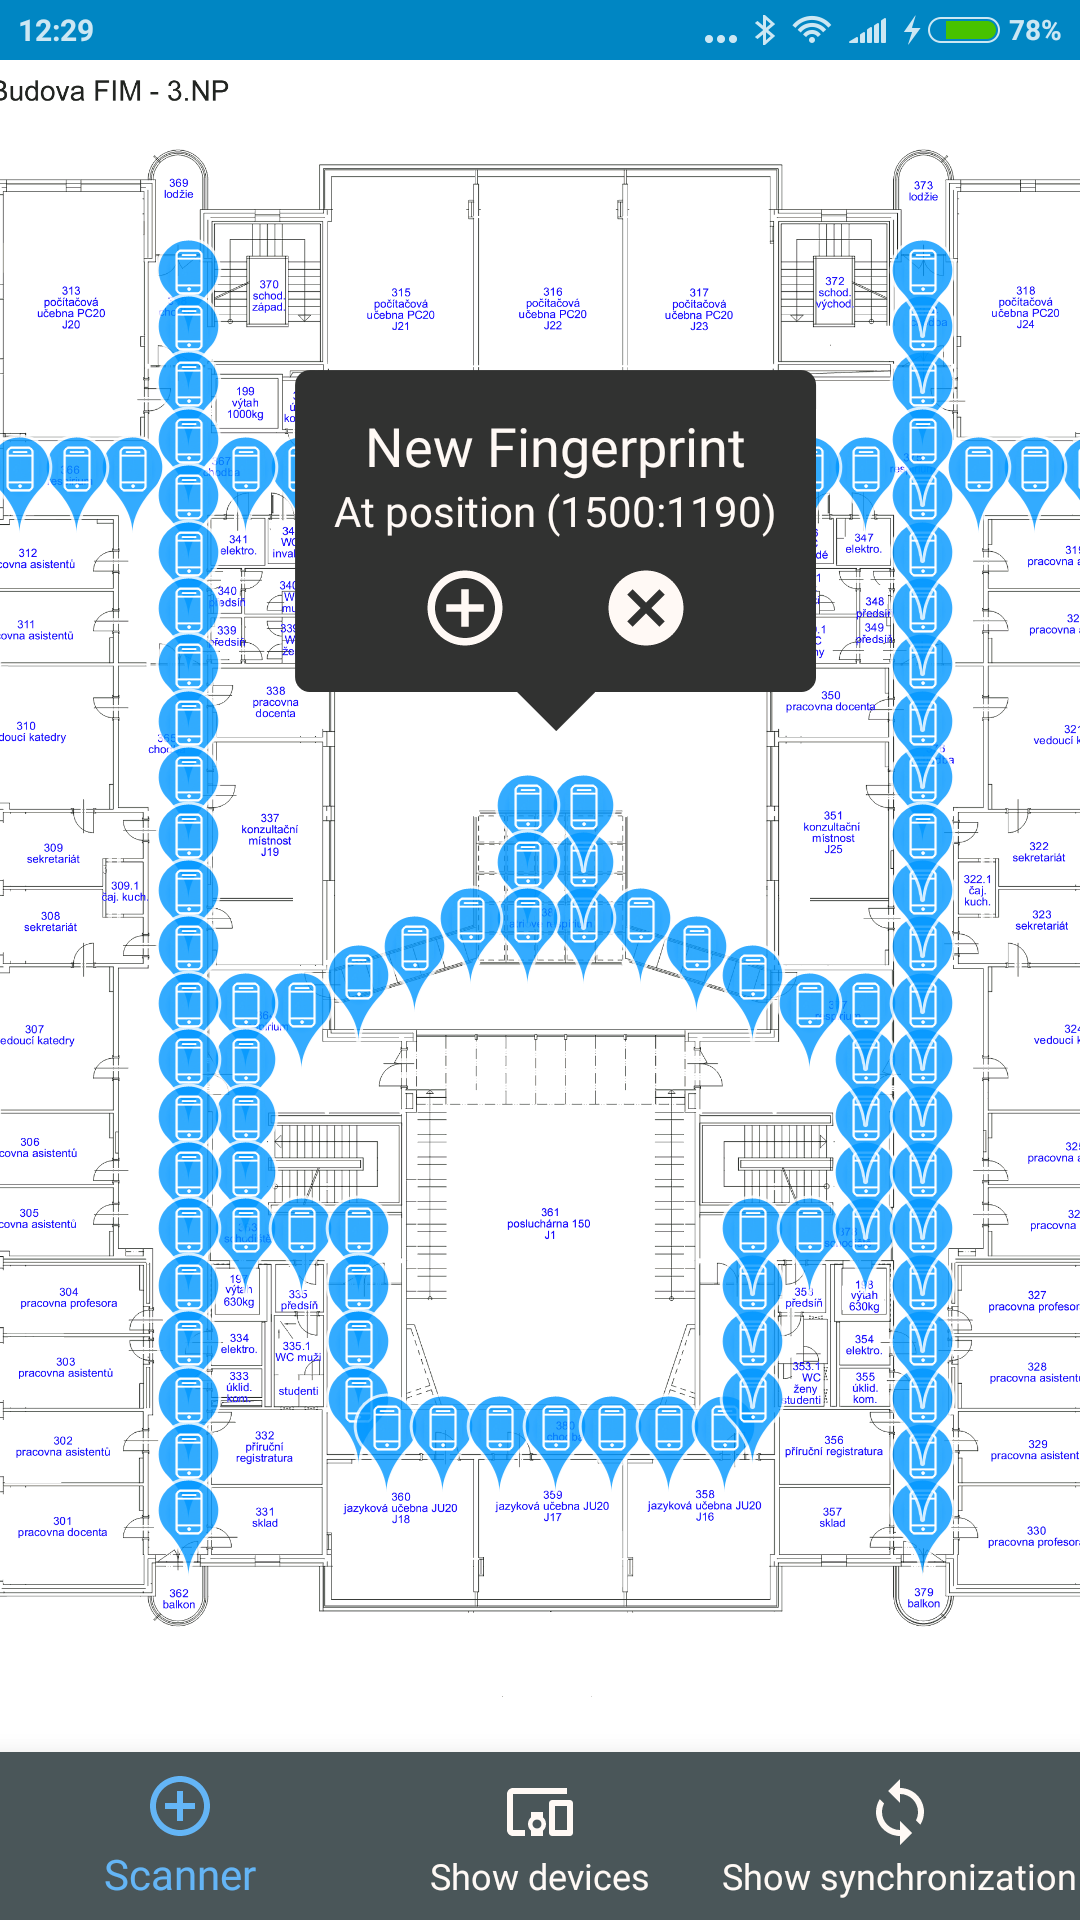
\includegraphics[width=0.30\textwidth]{img/map_markers}
		\hspace{0.2cm}
		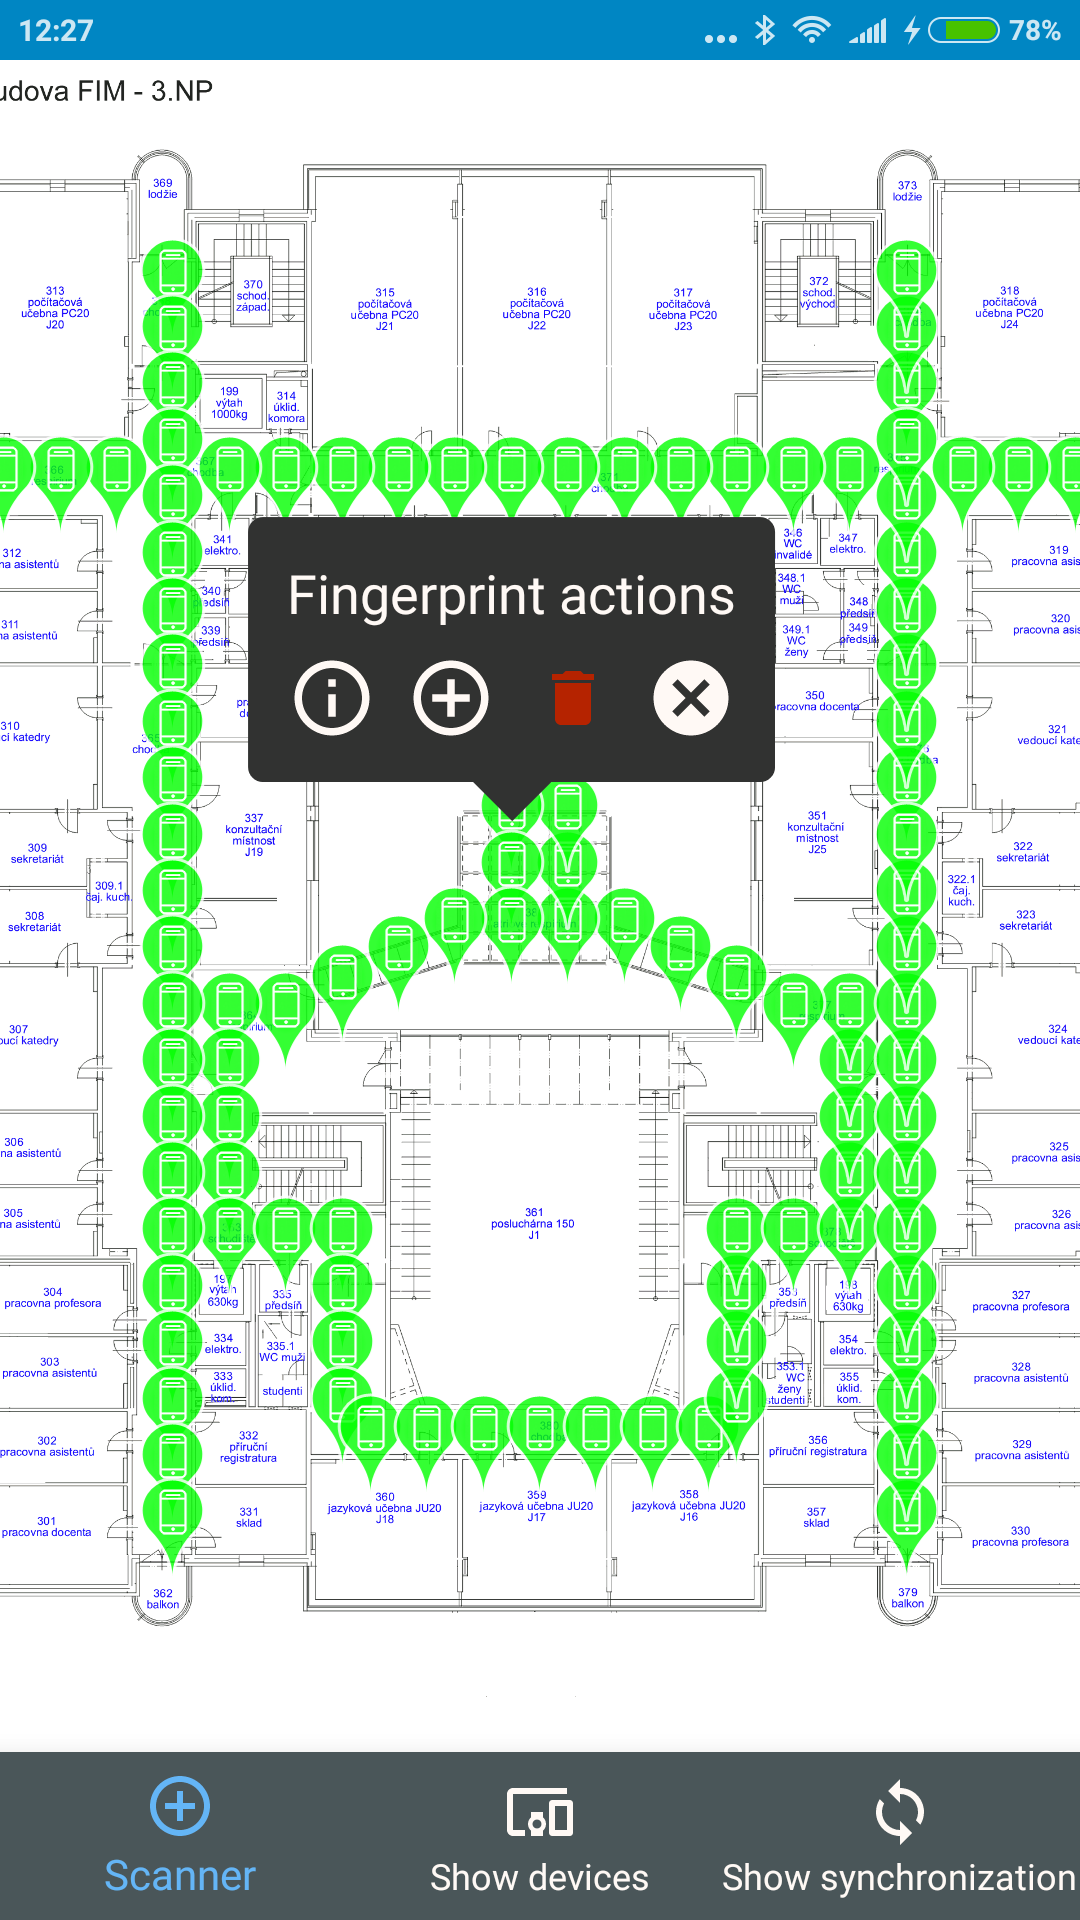
\includegraphics[width=0.30\textwidth]{img/map_markers_own}
		\par\end{centering}
	\caption{Map screen with markers\label{fig:map_with_markers}}
	\label{fig04c05}
\end{figure}

\fref{fig04c05} shows two screens of the map with markers, which are split by two colors and images. Color combination signifies if the latest fingerprint is from current device (green) or from another one (blue). This is based on fingerprint origin device, which is always mobile, meaning if wear displays as green then fingerprint originated on wear connected to the current mobile phone. Images combination distinguishes between device type, mobile and wear in this case.

Each spot on the map can be clicked, including the markers, to display overlay with fingerprint actions. There are two different displays for this overlay. First, when user clicks on existing marker there are options to display information about that specific spot, containing list of the fingerprints, enable user to create new fingerprint on that spot, delete last group or hide this window. Second, displayed when clicked spot does not have previously created fingerprints. This overlay displays only option to add new fingerprint or hide the window. Both of these options are displayed in \fref{fig04c05}.

Adding new fingerprints will create all necessary data for the scan and run it via already mentioned JobScheduler. This scan has always priority, meaning if there is a non-priority scan running it is canceled and this one is run instead. It can happen when devices screen initiated a scan which did not finish before scheduling a scan using this screen. When scan is running all application screens (Activities) display scan information as shown in the \fref{fig05c05}, thus informing about scan status in all parts of the application.

\begin{figure}[H]
	\begin{centering}
		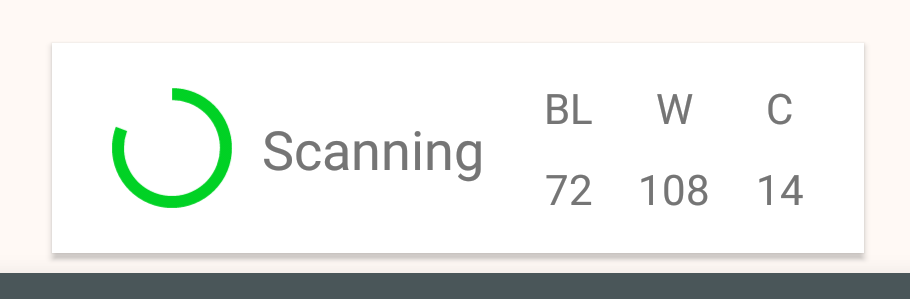
\includegraphics[width=0.6\textwidth]{img/scan_status}
		\par\end{centering}
	\caption{Scan status}
	\label{fig05c05}
\end{figure}

This information window overlays the screen just above the application menu. It informs user about scan status, progress and how many device records were saved until now. Informations displayed are BLE (B), WiFi (W) and Cellular (C) data collected but it does not show Sensor (S) information to save screen space.

Original map image has 3000x2200 pixels but with a low data size around 230 KB, so it could be displayed as a single image but for already mentioned reasons it is not. The image is cut into four zoom levels (1 to 4) with first having 4 images and the final one with 144. Left side of \fref{fig06c05} shows maximum zoom on the mobile screen and right side displays information about fingerprints in a specific spot.

\begin{figure}[h!]
	\begin{centering}
		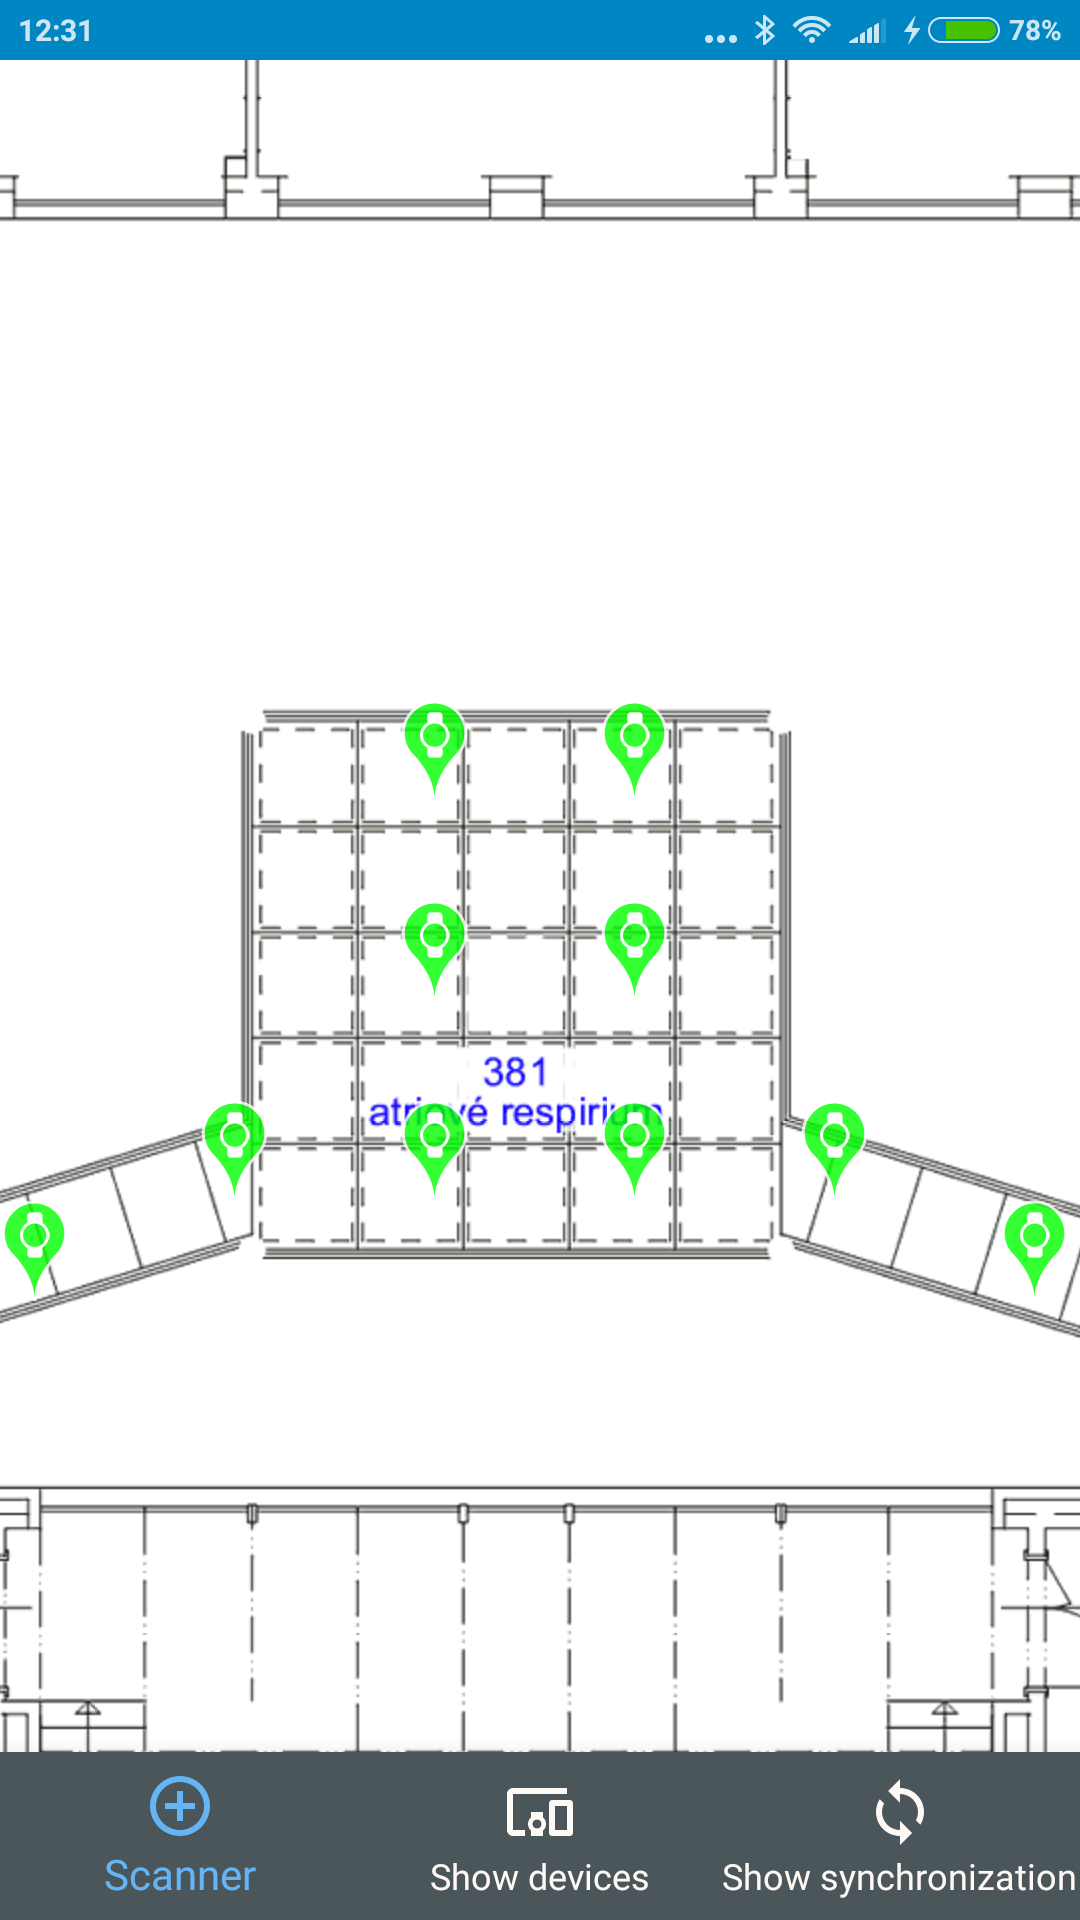
\includegraphics[width=0.30\textwidth]{img/map_zoom}
		\hspace{0.2cm}
		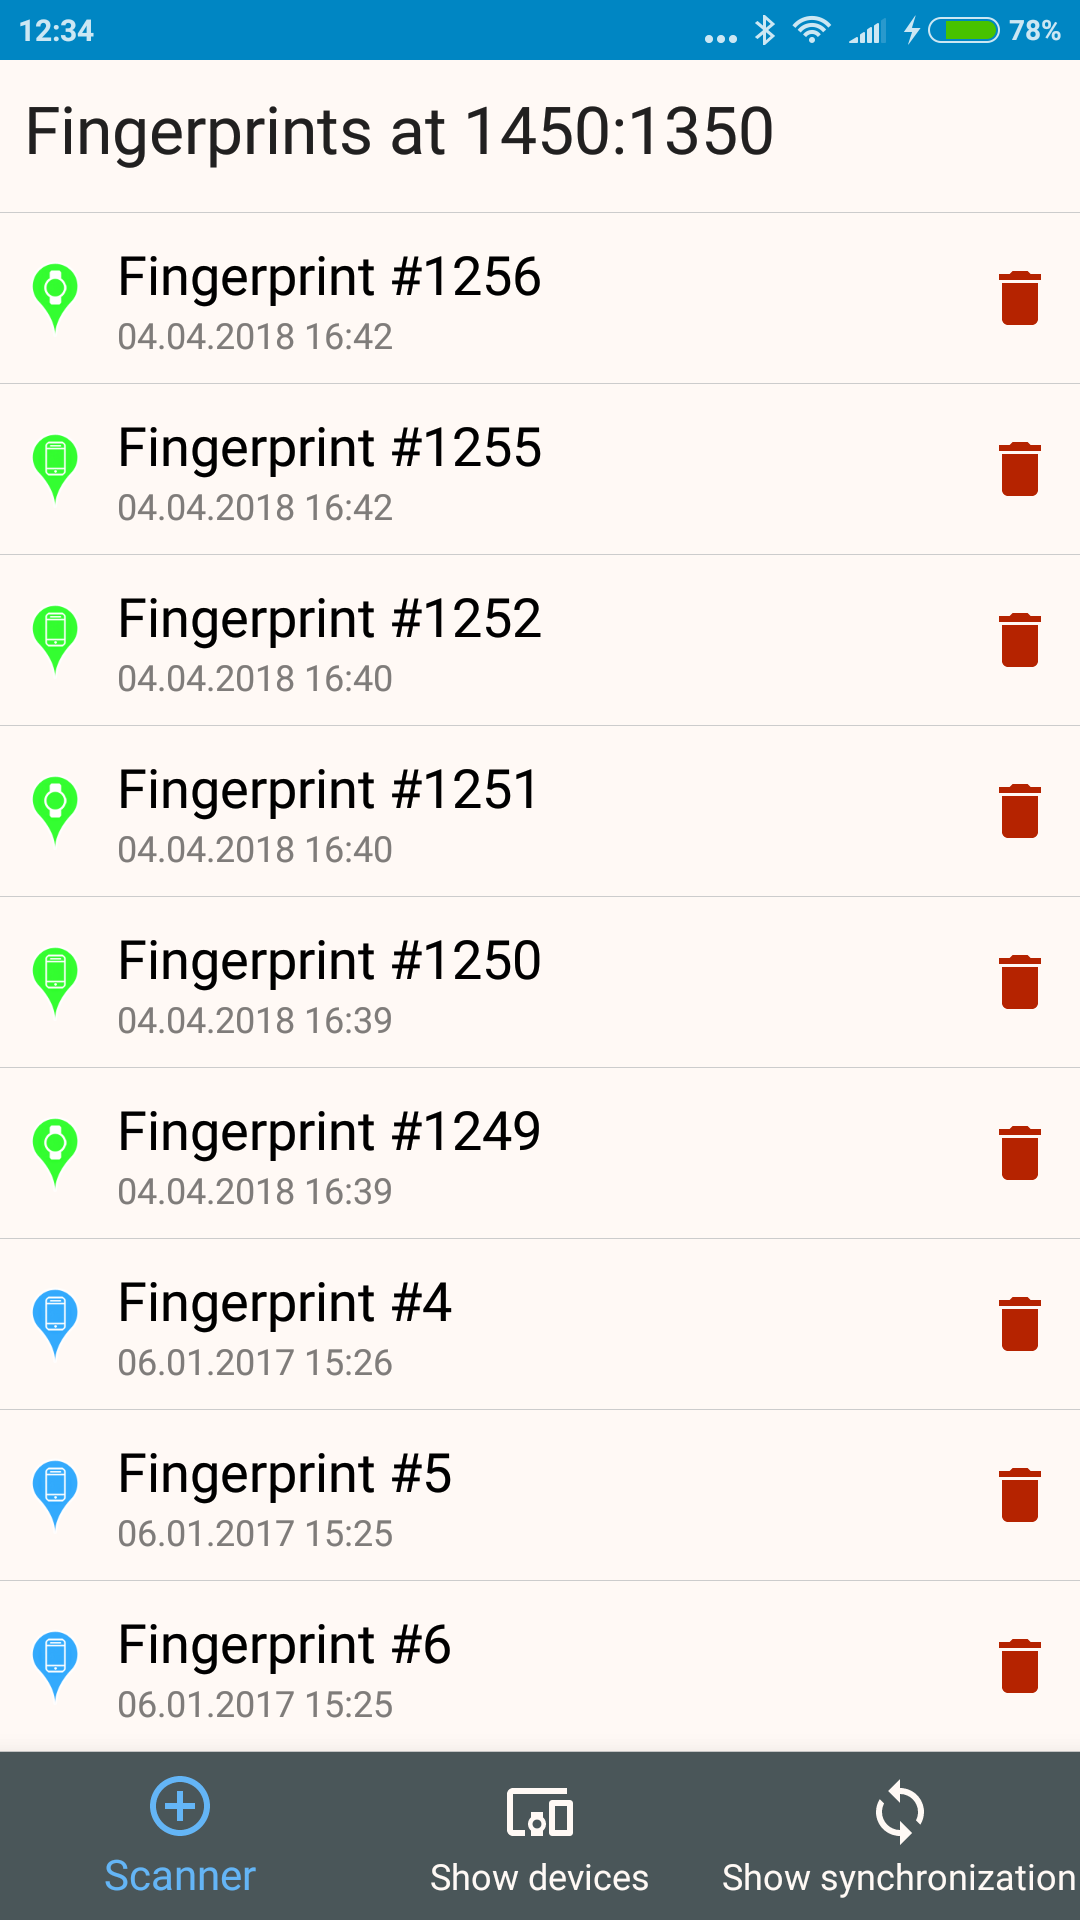
\includegraphics[width=0.30\textwidth]{img/map_list_fingerprints}
		\par\end{centering}
	\caption{Maximum map zoom (left), List of fingerprints (right)\label{fig:map_zoom_and_list}}
	\label{fig06c05}
\end{figure}

List of fingerprints for a specific spot displays information about origin device by icon, time it was created and enables to delete specific ones from the mobile. It is planned to extend this feature to display all important information about fingerprint, such as ids, device, counts of measurements and even RSSI averages. This would enable to assess fingerprint viability before uploading it on the server.

Important thing to note is that deleting fingerprints will not be reported to the server, therefore deletion of fingerprints is advised before uploading to the server. Deleting of already uploaded fingerprint on the phone will remove it only from that device and to delete it from the server is only enabled on the server itself. 

\subsubsection{Devices}\label{subsec:Devices}
This screen was supposed to be used for establishing connection between mobile and wearable device but this is done via WearOS application and not necessarily required since Data Layer API can now also send data between devices via WiFi. Even though it has no real use it was kept to display surrounding devices and mainly BLE beacons.

\begin{figure}[h!]
	\begin{centering}
		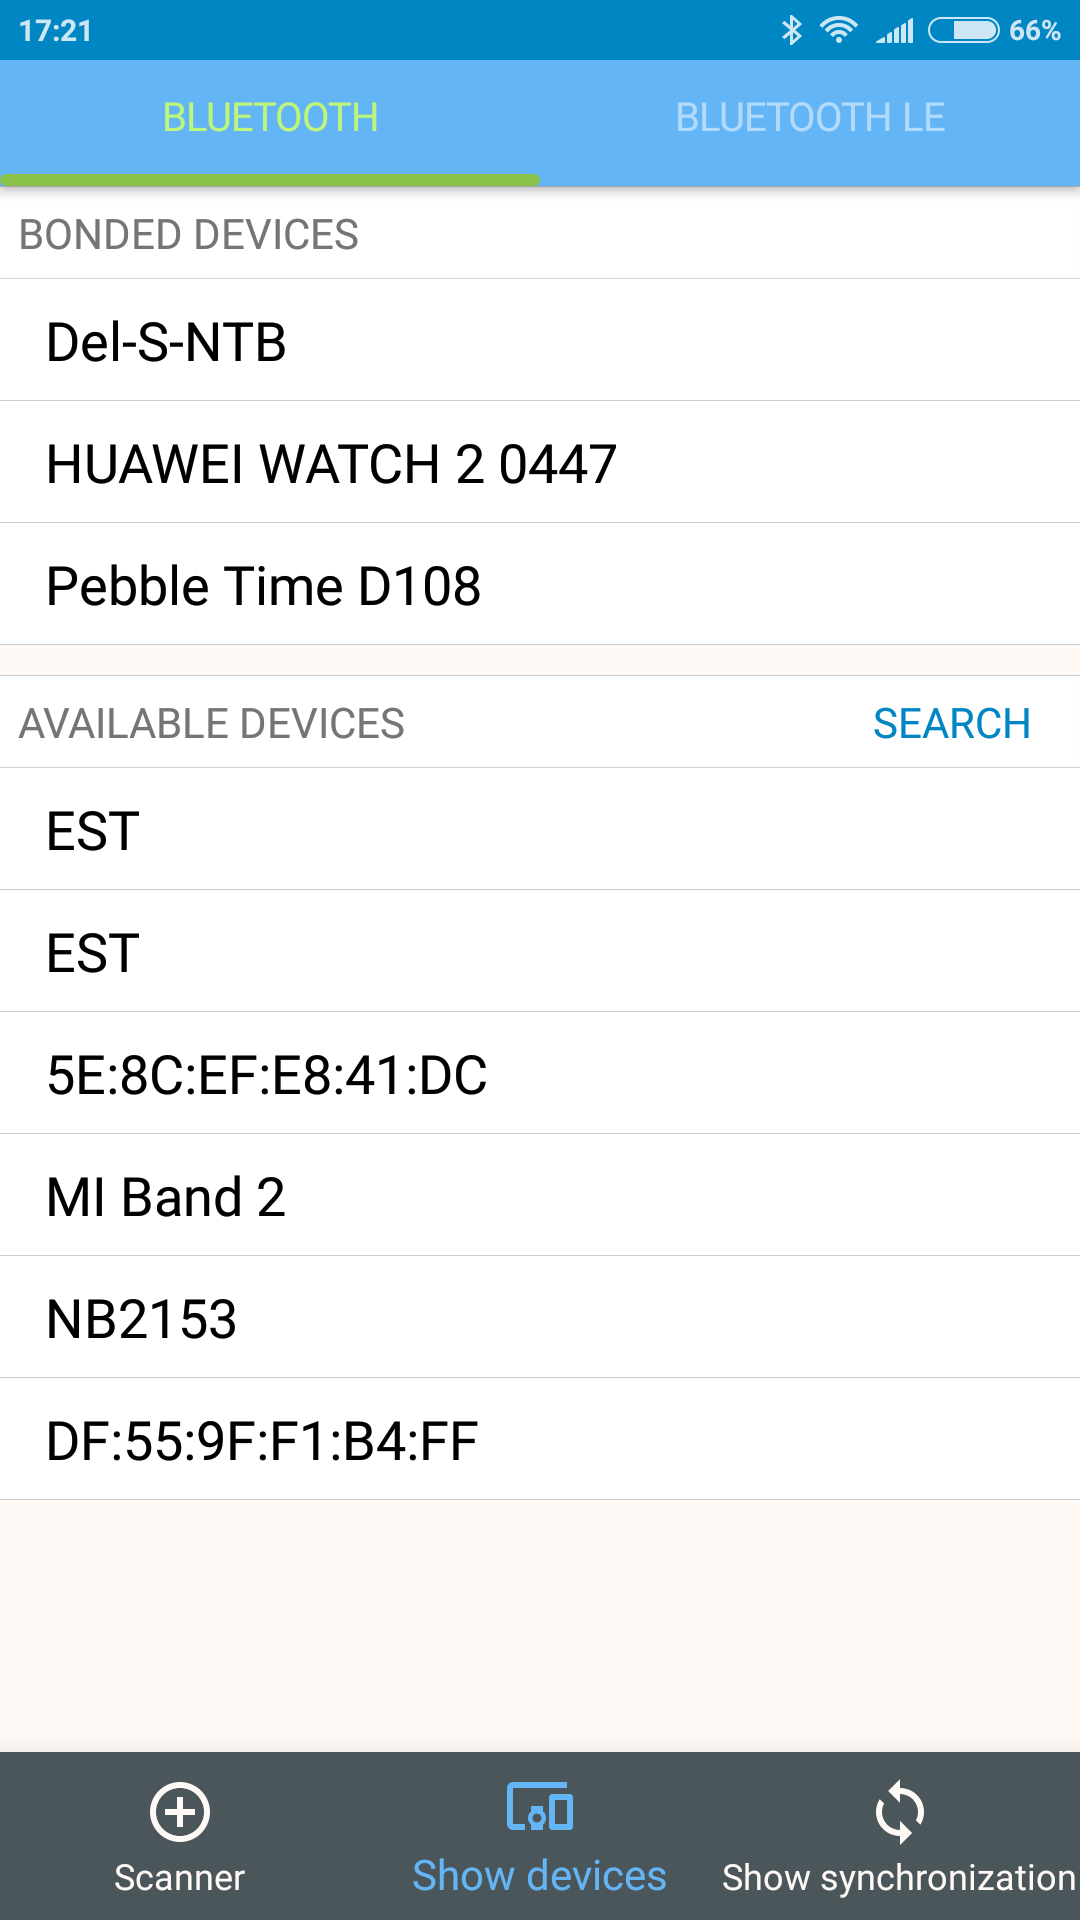
\includegraphics[width=0.30\textwidth]{img/devices_bl}
		\hspace{0.2cm}
		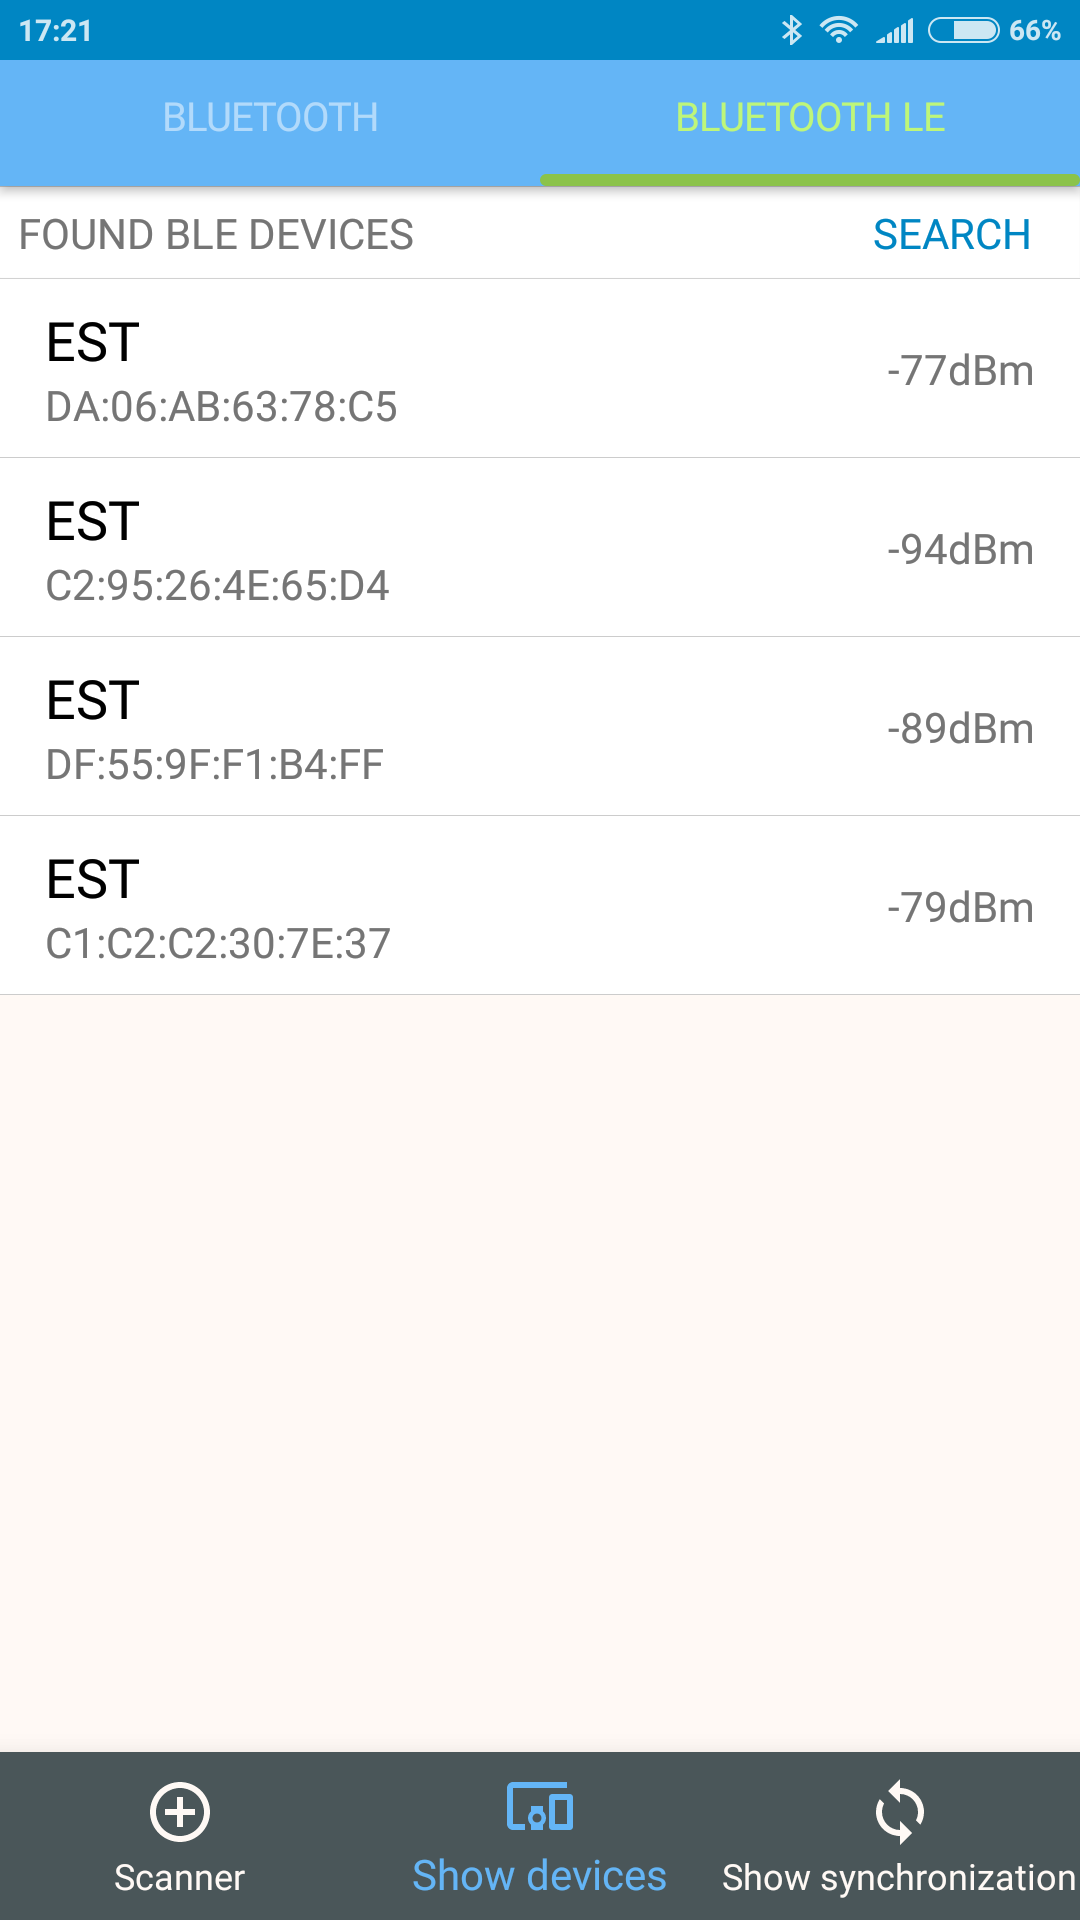
\includegraphics[width=0.30\textwidth]{img/devices_ble}
		\par\end{centering}
	\caption{Bluetooth devices (left), Beacons (right)\label{fig:bl_ble_list}}
	\label{fig07c05}
\end{figure}

Left screen of \fref{fig06c05} displays all the Bluetooth devices recorded during the last scan, which is 15 seconds long. This scanning feature is not continuous and to display new devices it is needed to start a new scan by pressing \enquote{Search} button, which will also clear the available devices list. There is no need to scan for bonded Bluetooth devices since Android keeps them in a separate list, which is good but it does not check if the devices are in range or not, this means it can also display the device that is not available.

Right screen displays only devices broadcasting using Bluetooth Low Energy, those are mainly beacons but it can also be wristbands, some TVs and few more devices. It displays basic information like name, mac address and last signal strength received. Same as Bluetooth scanning it is not continuous and initiated by pressing \enquote{Search} button where length of such scan is set to 30 seconds in this case.

There is a possibility, for both screens, of device not having the name set and if that is the case, mac address is displayed instead of a missing name. To make this screen more viable it could display more information about devices, plus it could be extended to show WiFi access-points and Cellular towers in range.

\subsubsection{Synchronization}\label{subsec:Synchronization}
As the name suggests this screen is used to synchronize data between mobile and the server. It shows current fingerprint differences and enables data synchronization based on used input. It does not download or upload the data on its own since it is very data consuming, that is why it needs to be triggered by the user. Contrary to scanning, it does not display information using an overlay with the status but it updates counts on the screen after every successful upload or download call is done. It also shows an animation of synchronization button on top of the screen and displays a message if synchronization finished successfully or failed to inform user about the status of this task.

\begin{figure}[H]
	\begin{centering}
		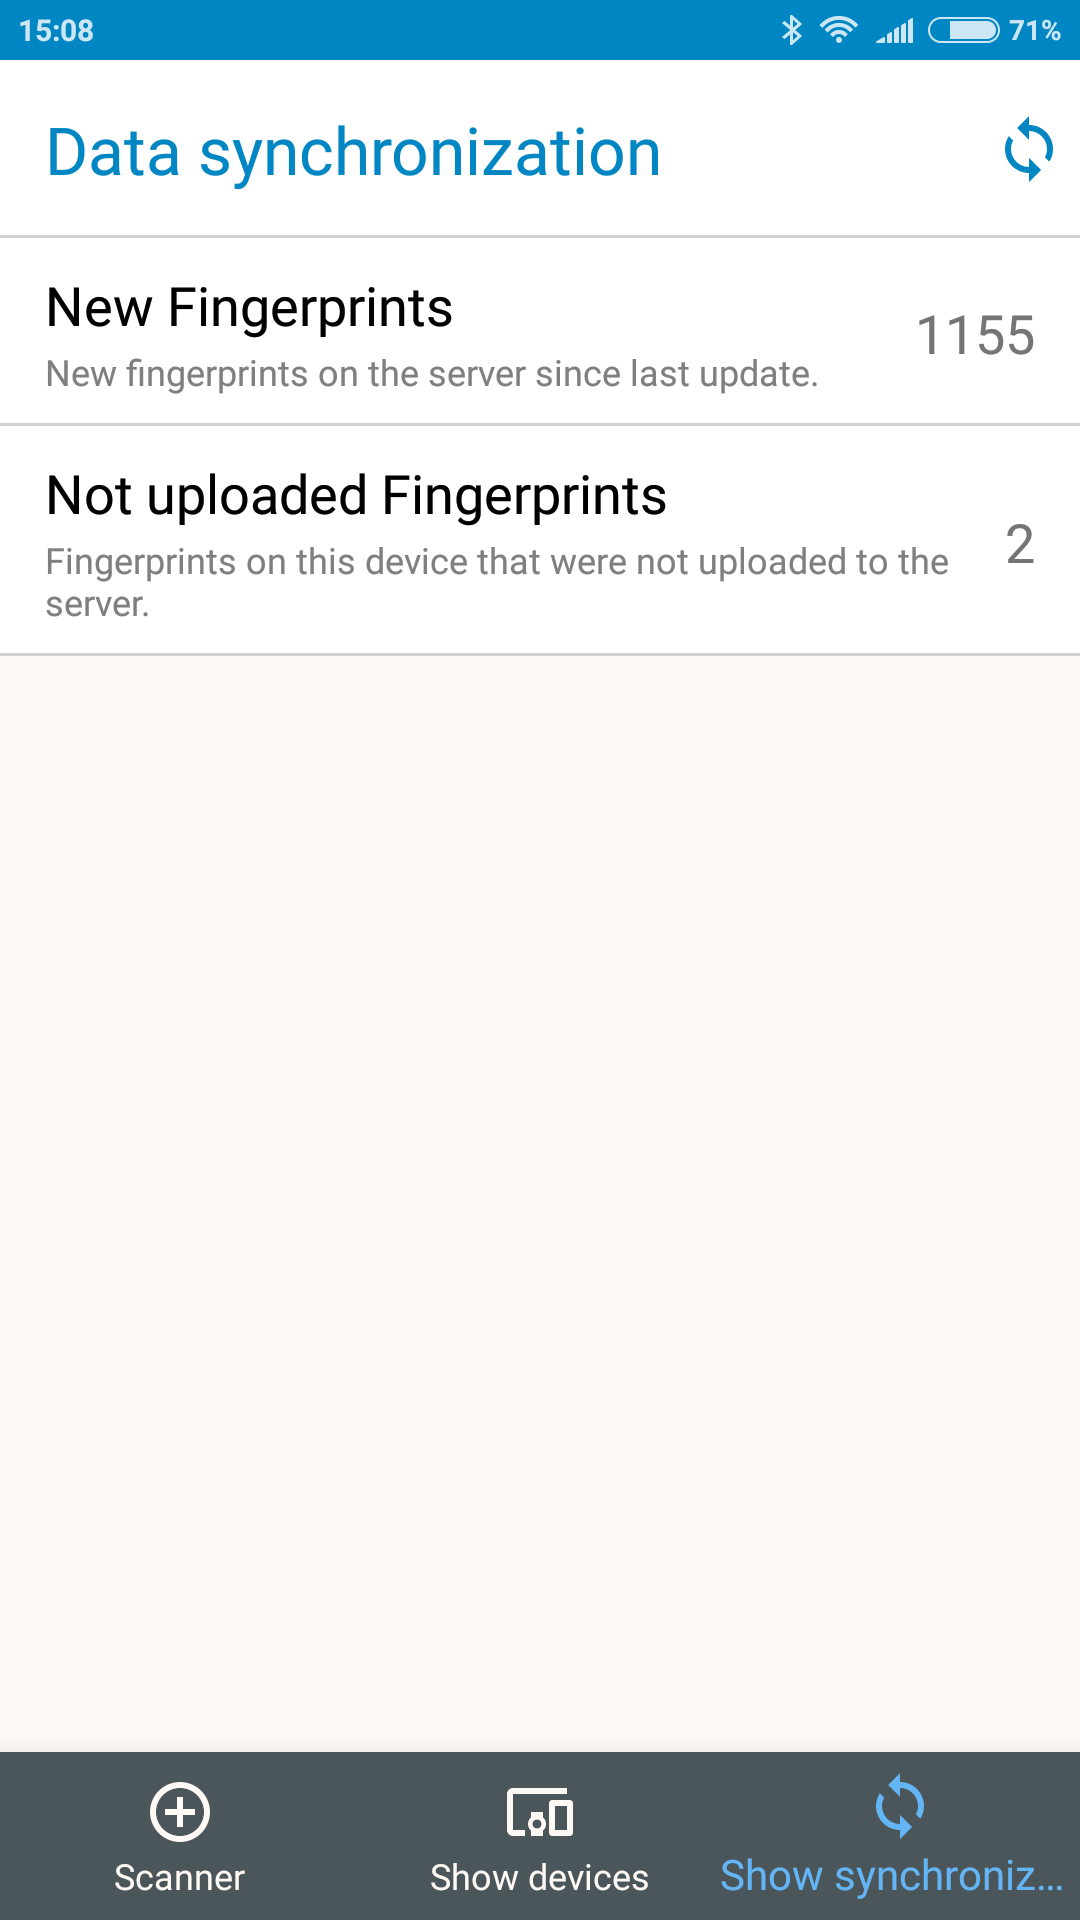
\includegraphics[width=0.3\textwidth]{img/synchronization}
		\par\end{centering}
	\caption{Synchronization screen}
	\label{fig08c05}
\end{figure}

It is planned to expand this screen for the use of application configuration to make it more flexible and able to be used in different environments than the current one. There are many changes considered which could influence the scanning results and application use.

\begin{itemize}
	\item Be able to change scanning properties like maximum length, time periods for each scan or make scanning periodic. There could also be separate settings for wearable device.
	\item Enable to change server API address and download/upload limits. The API would have to implement same endpoints as current one in this case.
	\item Implement map tiles uploading for different floors or buildings with the possibility to change between them and download fingerprints based on such selected location.
	\item User verification for the application and API with the possibility to change them on this screen.
\end{itemize}

\subsubsection{Wear scanner}\label{subsec:WearableScanner}
Wearable application is meant to be as simple as possible. It has only single screen since all the other settings are done on mobile application. This screen has two display states and holds the device wake lock preventing screen dimming or turning off when there is a scan running. Only reason to keep this wake lock is to display scan information without the need to click on wear screen. This feature could be also implemented as optional with the possibility to change in the phone application settings (currently synchronization) screen. 

\begin{figure}[H]
	\begin{centering}
		
\includegraphics[width=0.25\textwidth]{img/wear_waiting_edited}
		\hspace{0.5cm}
		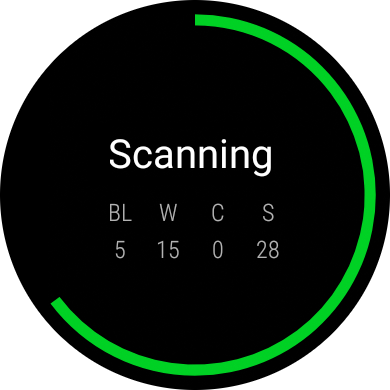
\includegraphics[width=0.25\textwidth]{img/wear_scanning_edited}
		\par\end{centering}
	\caption{Wear scanning screens}
	\label{fig09c05}
\end{figure}

First screen shows information message about receiving fingerprint data from mobile, when no data is received for 10 seconds it is closed to reduce battery drain. Second screen displays scan status with the progress bar and count of scanned records. When scan completes this informations stays displayed for tree seconds, after this time the screen is reset to the first one and application is closed. Since the scan can be run with wear at a position where user is not able to check the data, it informs about scan start and end with a short device vibration.

\subsection{Interesting code examples}\label{subsec:Interesting code examples}
This application is a collection of complex code and functions where some interesting parts were selected and described in more detail.

\subsubsection{Sending Fingerprint to Wear}\label{subsubsec:SendingFingerprintToWear}
Core functionality of communication between both devices. This code can be found in a WearDataSender class of mobile application and it sends fingerprint data to the wear using Data Layer API right after wear application is started.

\begin{lstlisting}[caption=Sending Fingerprint to Wear]
if(mFingerprint != null) {
	mFingerprint.setDeviceEntry(null);
	
	PutDataMapRequest dataMapRequest = PutDataMapRequest.create(DataLayerListenerService.SCAN_PATH);
	DataMap dataMap = dataMapRequest.getDataMap();
	ParcelableUtils.putParcelable(dataMap, DataLayerListenerService.SCAN_DATA, mFingerprint);
	
	PutDataRequest request = dataMapRequest.asPutDataRequest();
	request.setUrgent();
	Wearable.getDataClient(mContext).putDataItem(request);
	
	mFingerprint = null;
}
\end{lstlisting}

This class handles starting of wear application and also sending fingerprint data, that is why it has a global variable for fingerprint data. Fist line of the code checks if this variable is not empty so it could be send to wear device. This code does only one change to the fingerprint before it is send, it removes origin device information to be filled in by the wear. When fingerprint is prepared it must be converted into Parcelable DataMap which is an object that is shared via Data Layer. This data is identified by a string key so application can save multiple objects into this map. Next part of the code creates a request using this data and sets its mode to urgent to ensure fast delivery to all devices that listen for it. Request is completed at this point and can be send via DataClient which is loaded from the class Wearable. Final line of code takes care of clearing the global variable containing fingerprint to prevent sending the same data multiple times.

Data Layer identifies all the data by a specific Uri and when the data is changed it sends an information to all devices, meaning each fingerprint must be different for sending notification about the data change to other devices. Luckily every fingerprint has its own specific id and scan id which is always different so this feature does not pose any problem to the data sending.

\subsubsection{Parsing beacon information}\label{subsubsec:ParsingBeaconInformation}
None of the scanner parts uses default classes to contain scanned information. With each custom class data must be parsed from the default ones during the scanning. Following code, taken from FingerprintScanner class, shows an example how to parse beacon data.

\begin{lstlisting}[caption=Parsing beacon information]
String bssid = beacon.getBluetoothAddress();

long scanTime = currentMillis - mStartTime;
if(scanTime == currentMillis) {
	scanTime = 0;
}
long scanDifference = calculateBeaconScanDifference(scanTime, bssid);

BeaconEntry newBeacon = new BeaconEntry();
newBeacon.setBssid(bssid);
newBeacon.setDistance((float) beacon.getDistance());
newBeacon.setRssi(beacon.getRssi());
newBeacon.setTimestamp(currentMillis);
newBeacon.setScanTime(scanTime);
newBeacon.setScanDifference(scanDifference);

return newBeacon;
\end{lstlisting}

First loaded information is device mac address because it is used to calculate time differences between last time this device was recorded and current time which is done in following part. After all time values are calculated BeaconEntry can be created containing all required data and immediately returned. Setting scanTime to 0 works as a protection against having it the same as currentMillis because start time of the scan might not have been set just yet. This is needed mainly for WiFi scanning because these parsing classes have to be set just before running the scanner code which leaves few milliseconds where data can be recorded before scan is actually stared, considering WiFi scan cannot be controlled. It could be also solved by not recording this data but since it is only few milliseconds difference it was decided that environment will not change enough to make the data irrelevant and so they are recorded too.

\subsubsection{Map configuration}\label{subsubsec:MapConfiguration}
Map is the main part of mobile application and it handles multiple functions thus requiring a lot of settings to work as intended. It also supports many functions which can be configured or disabled based on the implementation required. This map and the code is implemented in MapFragment class and displayed using MapActivity.

\begin{lstlisting}[caption=Map configuration]
mMap.setSize(MAP_WIDTH, MAP_HEIGHT);
mMap.addDetailLevel(1.000f, "tiles/j3np/1000/j3np-%d_%d.png");
mMap.addDetailLevel(0.500f, "tiles/j3np/500/j3np-%d_%d.png");
mMap.addDetailLevel(0.250f, "tiles/j3np/250/j3np-%d_%d.png");
mMap.addDetailLevel(0.125f, "tiles/j3np/125/j3np-%d_%d.png");

mMap.setScaleLimits(0, 2); 
mMap.setScale(0.50F);

... Setup markers and hotspots ...

frameTo(MAP_WIDTH / 2, MAP_HEIGHT / 2);

mMap.setShouldRenderWhilePanning(true);
mMap.setShouldLoopScale(false);
\end{lstlisting}

First part contains setting map size which is 3000x3000 pixels and configure zoom levels with their specific tile images based on given path. Setting zoom levels one by one makes it highly modifiable with the possibility to have different designs for each zoom level. Next part sets zoom values, such as allowed zoom levels and initial zoom of the map. Following part is setting up markers and hotspots which will be described later. Calling function \verb|frameTo()| centers the map with a delay because if it is done immediately it does not work. Final part of this code enables loading when map is panning and disables returning to maximum zoom level after double clicking while being zoomed in, on zoom level 2 in this case.

\begin{lstlisting}[caption=Setup markers and hotspots]
mMap.setMarkerTapListener(mMarkerTapListener);
mMap.defineBounds(0, 0, MAP_WIDTH, MAP_HEIGHT);
mMap.setMarkerAnchorPoints(-0.5f, -0.5f);

HotSpot hotSpot = new HotSpot();
hotSpot.set(0, 0, MAP_WIDTH, MAP_HEIGHT);
mMap.addHotSpot(hotSpot);
mMap.setHotSpotTapListener(mHotspotTapListener);
\end{lstlisting}

This code example sets variables for map markers, such as displaying control window after clicking, define bounds and anchor point for marker centering it horizontally and vertically. Defining bounds to the markers is very important information because it enables to calculate real pixel location from map's absolute position because location of map markers changes based on how much the map is zoomed in. Scanner needs the real marker location to create fingerprint on the right spot and thus enabling the localization evaluation. This code does not actually display any markers on the map, that is done later in the code.

Second part of this example works similarly to previous one but it does not set the click function only to markers but creates an invisible overlay over the whole map, thus effectively enabling to click on any part of the map to display control window for fingerprints.
\chapter{Testing and data analysis}\label{sec:TestingAndDataAnalysis}
This chapter goal is to show application testing, data collection and analysis.

\section{Data collection}
\label{sec:DataCollection}

\section{Analysis}
\label{sec:Analysis}
\chapter{Conclusion}\label{sec:Conclusion}
This thesis has introduced a new way to collect radio fingerprints on mobile in combination with wear device to improve indoor stationary localization. This solution also included changes to data distribution between devices and the server. Created system consists of a server, mobile and wear devices with the Android operating system and WearOS for wear, both of them with Bluetooth Low Energy support. This system is designed to enable creation of radio fingerprint maps and update them anytime. Evaluation of this system was based on the Weighted K-Nearest Neighbors algorithm. This evaluation works only with specifically defined beacons and WiFi access-points to maintain equal environment for all fingerprints. Based on the acquired data in a real world scenario, the results of the localization were evaluated using WiFi, BLE and their combination with addition to using data from mobile, wear and their combination.

Evaluation was composed of three main algorithm implementations to figure out how to use data from multiple device types to improve overall localization accuracy. First test, using data from all device types separately showed lower accuracy of WiFi localization on wear, this was traced back to wear device not possessing the ability to scan for 5 GHz WiFi signals. This actually makes overall localization less accurate when combining the data together, where mean error increased from 0.85 to 1.52 meters, making it almost two times worse. Second test used one fingerprint per device type and averaged their location resulting in improvement of overall accuracy compared to previous evaluation but it is still not as precise and using single mobile device. Third and final evaluation combined data from multiple fingerprints at the same position and created using different device types, data from wear are cloned into data from mobile fingerprints.

Best results were reached when combining fingerprint data from both devices into a single one with up to 6\% improvement of overall accuracy which should be even higher in locations not using 5 GHz WiFi networks. When this network is used and wear device does not support them, it is better not to include WiFi data from wear in the evaluation.

It was proved that wear device can improve localization when used with the mobile but it is important to keep in mind that at this time smartwatches do not possess high battery life and cannot be used to scan for a long period of time. Higher battery life could also mean the possibility for manufacturers to implement 5 GHz WiFi receiver and effectively improve localization bringing accuracy to the level of mobile device. Important thing to mention is that smartwatch localization can sometimes be preferred since it is tightly connected to a person.

\subsection{Future improvements}\label{sec:FutureImprovements}
This application is meant to be used in different environments and the first improvement should be to enable uploading of new maps and differentiating between locations, make it possible to change between them and load different fingerprints based on a specific location. Another likely improvement is making scanning more viable by supporting changes in its settings like length of the scan or lengths of all sub-scans. Final and very important improvement could be implementation of location calculation and display, where scanned data would be send to the server which would return calculated location to the application. This part would be implemented at the end of development process or it could be implemented in a separate solution to prevent over-compilation of existing application.

\begin{thebibliography}{10}

\bibitem{GNSS}
Bernhard Hofmann-Wellenhof, Herbert Lichtenegger and Elmar Wasle. \textit{GNSS – Global Navigation Satellite Systems: GPS, GLONASS, Galileo, and more}. Springer Science \& Business Media, 2007 [cited 2018-01-10], ISBN 9783211730171.

\bibitem{GNSSGPS}
AviationChief. \textit{Global Navigation Satellite System (GNSS) Global Positioning Satellite (GPS) System} [online]. AviationChief.Com, 2017 [cited 2018-01-15]. Available at: \url{http://www.aviationchief.com/gps-system.html}

\bibitem{LocalizationApproaches}
Xinglin Piao, Yong Zhang, Tingshu Li, Yongli Hu, Hao Liu, Ke Zhang and Yun Ge. \textit{RSS Fingerprint Based Indoor Localization Using Sparse Representation with Spatio-Temporal Constraint} [online]. National Center for Biotechnology Information, 2016 [cited 2018-01-14], Available at: \url{https://www.ncbi.nlm.nih.gov/pmc/articles/PMC5134504/}

\bibitem{PedestrianDeadReckoning}
Stéphane Beauregard and Harald Haas. \textit{Pedestrian Dead Reckoning: Basis for Personal Positioning} [online]. School of Engineering and Science
International University Bremen, 2006, Available at: \url{http://ave.dee.isep.ipp.pt/~lbf/PINSFUSION/BeHa06.pdf}

\bibitem{AaPLocalisation}
Gabriel Deak, Kevin Curran and Joan Condell. \textit{A survey of active and passive indoor localisation systems}. In: \textit{Computer Communications}. Elsevier, 2012 [cited 2018-01-11], Volume 35, Issue 16, ISSN: 0140-3664.

\bibitem{RAinWILTaS}
Zahid Farid, Rosdiadee Nordin, and Mahamod Ismail. \textit{Recent Advances in Wireless Indoor Localization Techniques and System} [online]. School of Electrical, Electronics \& System Engineering, University Kebangsaan Malaysia (UKM), 2013 [cited 2018-01-15], Available at: \url{http://downloads.hindawi.com/journals/jcnc/2013/185138.pdf}

\bibitem{LTinWSN}
Shweta Singh, Ravi Shakya and Yaduvir Singh. \textit{Localization techniques in wireless sensor networks} [online]. Department of Computer Science,
Ideal Institute of Technology, Ghaziabad, 2015 [cited 2018-01-15], ISSN: 0975-9646, Available at: \url{https://pdfs.semanticscholar.org/6299/85defbf9cc1a937a1b88c9c2a893552e3d89.pdf}

\bibitem{AoALforWSN}
Paweł Kułakowski, Javier Vales-Alonso, Esteban Egea-López, Wiesław Ludwin and Joan García-Haro. \textit{Angle-of-arrival localization based on antenna arrays for wireless sensor networks} [online]. In: \textit{Computers \& Electrical Engineering}. Elsevier, 2010 [cited 2018-01-15], Volume 36, Issue 6, Pages 1181-1186. Available at: \url{http://ai2-s2-pdfs.s3.amazonaws.com/17c6/0e17c4e72cc3fd821e12169c1c2ca7736bd4.pdf}

\bibitem{IILUBLEB}
Pavel Kriz, Filip Maly, and Tomas Kozel. \textit{Improving Indoor Localization Using Bluetooth Low Energy Beacons} [online]. In: \textit{Mobile Information Systems}. Hindawi Publishing Corporation, 2016 [cited 2018-01-15], Volume 2016, Article ID 2083094. Available at: \url{https://www.hindawi.com/journals/misy/2016/2083094/abs/}

\bibitem{TvTHGPSRW}
GISGeography. \textit{Trilateration vs Triangulation – How GPS Receivers Work} [online]. GISGeography.com, 2018 [cited 2018-01-15]. Available at: \url{http://gisgeography.com/trilateration-triangulation-gps/}

\bibitem{HPwAA}
Kenjirou Fujii, Yoshihiro Sakamoto, Wei Wang, Hiroaki Arie, Alexander Schmitz and Shigeki Sugano. \textit{Hyperbolic Positioning with Antenna Arrays and Multi-Channel Pseudolite for Indoor Localization} [online]. MDPI AG, Basel, 2015 [cited 2018-01-15]. Available at: \url{http://www.mdpi.com/1424-8220/15/10/25157/htm}

\bibitem{PLTaA}
David Munoz, Frantz Bouchereau Lara, Cesar Vargas and Rogerio Enriquez-Caldera. \textit{Position Location Techniques and Applications}. Elsevier Science Publishing Co Inc, 2009 [cited 2018-01-15], ISBN: 9780080921938. Available at: \url{http://www.mdpi.com/1424-8220/15/10/25157/htm}

\bibitem{AoA}
Group 891: Wireless Location. \textit{ANGULATION: AOA (Angle Of Arrival)} [online]. DEPARTMENT OF ELECTRONIC SYSTEMS, Aalborg University, 2010 [cited 2018-01-15]. Available at: \url{http://kom.aau.dk/group/10gr891/methods/Triangulation/Angulation/ANGULATION.pdf}

\bibitem{RofAoA}
Jais, M. I., Ehkan, P., Ahmad, R. B., Ismail, I., Sabapathy, T., and Jusoh, M. \textit{Review of angle of arrival (AOA) estimations through received signal strength indication (RSSI) for wireless sensors network (WSN)} [online]. In: Computer, Communications, and Control Technology (I4CT), 2015 International Conference on. IEEE, 2015, [cited 2018-01-16], p. 354-359. Available at: \url{https://www.researchgate.net/profile/Phaklen_Ehkan/publication/283476641_Review_of_angle_of_arrival_AOA_estimations_through_received_signal_strength_indication_RSSI_for_wireless_sensors_network_WSN/links/564106b008aebaaea1f6d6e5/Review-of-angle-of-arrival-AOA-estimations-through-received-signal-strength-indication-RSSI-for-wireless-sensors-network-WSN.pdf}

\bibitem{QAoA}
Quuppa Oy. \textit{Quuppa Intelligent Locating System} [online]. 2018 [cited 2018-01-16]. Available at: \url{http://quuppa.com/technology/}

\bibitem{ILWTP}
Krishna Chintalapudi, Anand Padmanabha Iyer, and Venkata N. Padmanabhan. \textit{Indoor Localization Without the Pain} [online]. In: Proceedings of the sixteenth annual international conference on Mobile computing and networking, 2010 [cited 2018-01-16], Available at: \url{http://dl.acm.org/citation.cfm?id=1860016}

\bibitem{RSSFofIFD}
Xiaoyang Wen, Wenyuan Tao, Chung-Ming Own, and Zhenjiang Pan. \textit{On the Dynamic RSS Feedbacks of Indoor Fingerprinting Databases for Localization Reliability Improvement} [online]. Sensors, 2016 [cited 2018-01-16], Available at: \url{https://www.ncbi.nlm.nih.gov/pmc/articles/PMC5017443/}

\bibitem{WiFiLBS}
Cisco. \textit{Wi-Fi Location-Based Services 4.1 Design Guide - Location Tracking Approaches} [online]. Cisco, 2018 [cited 2018-01-16], Available at: \url{https://www.cisco.com/c/en/us/td/docs/solutions/Enterprise/Mobility/WiFiLBS-DG/wifich2.html}

\bibitem{LSfUC}
Jeffrey Hightower and Gaetano Borriello. \textit{Location systems for ubiquitous computing} [online]. Computer, 2001 [cited 2018-01-17], 34.8: 57-66. Available at: \url{http://www.csd.uoc.gr/~hy439/lectures11/hightower2001survey.pdf}

\bibitem{LSAWIFI}
COOK, B., et al. \textit{Location by scene analysis of wi-fi characteristics} [online]. Relation, 2009 [cited 2018-01-17], 10.1.119: 6216. Available at: \url{http://www.ee.ucl.ac.uk/lcs/previous/LCS2006/2.pdf}

\bibitem{DRNS}
Levi, R.W. and Judd, T. \textit{Dead reckoning navigational system using accelerometer to measure foot impacts} [online]. Google Patents, 1996 [cited 2018-01-17]. Available at: \url{https://www.google.com/patents/US5583776}

\bibitem{IDRAIP}
Z. Zhou, T. Chen, L. Xu. \textit{An Improved Dead Reckoning Algorithm for Indoor Positioning Based on Inertial Sensors} [online]. In: Advances in Engineering Research, 2015 [cited 2018-01-17]. ISBN: 978-94-62520-71-4. Available at: \url{https://www.atlantis-press.com/proceedings/eame-15/22314}

\bibitem{IPBLEIUMWD}
NAKAJIMA, Naoki, et al. \textit{Improving Precision of BLE-based Indoor Positioning by Using Multiple Wearable Devices} [online]. In: Adjunct Proceedings of the 13th International Conference on Mobile and Ubiquitous Systems: Computing Networking and Services. ACM, 2016 [cited 2018-03-26]. p. 118-123. Available at: \url{https://dl.acm.org/citation.cfm?id=3004041}

\bibitem{SmartFix}
WANG, Xiaoliang; XU, Ke; LI, Ziwei. \textit{SmartFix: Indoor Locating Optimization Algorithm for Energy-Constrained Wearable Devices.} In: Wireless Communications and Mobile Computing, 2017 [cited 2018-03-26]. Available at: \url{https://dl.acm.org/citation.cfm?id=3004041}

\bibitem{TinyLoc}
W. Xiaoliang, X. Ke, Y. Zheng, and Z. Ge. \textit{Tinyloc: Indoor localization for energy-constrained wearable devices} [online]. In: Chinese Journal of Computers, 2016 (Chinese), [cited 2018-03-26]. Available at: \url{http://www.cnki.net/kcms/detail/11.1826.TP.20161106.1649.002.html}

\bibitem{MoLoc}
SUN, Wei, et al. \textit{MoLoc: On distinguishing fingerprint twins} [online]. In: Distributed Computing Systems (ICDCS), 2013 IEEE 33rd International Conference on. IEEE, 2013 [cited 2018-03-26]. p. 226-235. Available at: \url{http://ieeexplore.ieee.org/abstract/document/6681592/}

\bibitem{SWvsSP}
HOELZL, Gerold, et al. \textit{Size does matter-positioning on the wrist a comparative study: Smartwatch vs. smartphone} [online]. In: Pervasive Computing and Communications Workshops (PerCom Workshops), 2017 IEEE International Conference on. IEEE, 2017 [cited 2018-03-30]. p. 703-708.

\bibitem{WIGA}
Marziah Karch. \textit{What Is Google Android?} [online]. Lifewire, 2017 [cited 2018-01-17]. Available at: \url{https://www.lifewire.com/what-is-google-android-1616887}

\bibitem{AOSP}
Android. \textit{Android Open Source Code} [online]. Android.com, 2018 [cited 2018-01-17]. Available at: \url{https://source.android.com/}

\bibitem{AD}
Android. \textit{Android Developers} [online]. Android.com, 2018 [cited 2018-01-17]. Available at: \url{https://developer.android.com/index.html}

\bibitem{UtCoAWO}
Renju Liu and Felix Xiaozhu Lin. \textit{Understanding the Characteristics of Android Wear OS} [online]. In: Proceedings of the 14th Annual International Conference on Mobile Systems, Applications, and Services. ACM, 2016. p. 151-164. Available at: \url{https://athena.smu.edu.sg/mobisys/backend/mobisys/assets/paper_list/pdf_version/paper_12.pdf}

\bibitem{MIWD}
Samuel Gibbs. \textit{10 most influential wearable devices} [online]. Guardian News, 2017 [cited 2018-01-18]. Available at: \url{https://www.theguardian.com/technology/2017/mar/03/10-most-influential-wearable-devices}

\bibitem{GSWWDS}
Gartner, Inc. \textit{Gartner Says Worldwide Wearable Device Sales to Grow 17 Percent in 2017} [online]. Gartner, Inc., 2017 [cited 2018-01-18]. Available at: \url{https://www.gartner.com/newsroom/id/3790965}

\bibitem{SoASTaD}
Bahman Rashidi and Carol Fung. \textit{A Survey of Android Security Threats and Defenses} [online]. JoWUA, 2015, [cited 2018-01-19]. Available at: \url{https://www.researchgate.net/profile/Bahman_Rashidi2/publication/282365848_A_Survey_of_Android_Security_Threats_and_Defenses/links/560ec06908ae6b29b499a51f/A-Survey-of-Android-Security-Threats-and-Defenses.pdf}

\bibitem{ASIMPD}
Parvez Faruki, Ammar Bharmal, Vijay Laxmi, Vijay Ganmoor, Manoj Singh Gaur and Mauro Conti. \textit{Android Security: A Survey of Issues, Malware Penetration and Defenses} [online]. IEEE Communications Surveys and Tutorials, 17(2), pp. 998-1022, 2015, [cited 2018-01-19]. Available at: \url{http://dx.doi.org/10.1109/COMST.2014.2386139}

\bibitem{NoAAiGPS}
Statista. \textit{Number of available applications in the Google Play Store from December 2009 to December 2017} [online]. Statista, 2018, [cited 2018-01-19]. Available at: \url{https://www.statista.com/statistics/266210/number-of-available-applications-in-the-google-play-store/}

\bibitem{NoAA}
AppBrain. \textit{Number of Android applications} [online]. AppBrain, 2018, [cited 2018-01-19]. Available at: \url{https://www.appbrain.com/stats/number-of-android-apps}

\bibitem{CSUITW}
LIU, Xing, et al. \textit{Characterizing Smartwatch Usage In The Wild} [online]. In: Proceedings of the 15th Annual International Conference on Mobile Systems, Applications, and Services. ACM, 2017 [cited 2018-01-19]. p. 385-398. Available at: \url{https://pdfs.semanticscholar.org/0cc2/4bccc3067ed688e576603bc6bab0e5e1b1db.pdf}

\bibitem{UCAW}
Liu, Renju, and Felix Xiaozhu Lin. \textit{Understanding the Characteristics of Android Wear OS} [online]. In: Proceedings of the 14th Annual International Conference on Mobile Systems, Applications, and Services. ACM, 2016 [cited 2018-01-19], p. 151-164. Available at: \url{https://athena.smu.edu.sg/mobisys/backend/mobisys/assets/paper_list/pdf_version/paper_12.pdf}

\bibitem{AWPaS}
Sandra Henshaw. \textit{Android Wear Problems (and Solutions!)} [online]. Tiger Mobiles Limited, 2016 [cited 2018-01-20]. Available at: \url{https://www.tigermobiles.com/2016/01/android-wear-problems-and-solutions/}

\bibitem{WAWP}
Simon Hill. \textit{10 of the worst Android Wear problems, and how to fix them} [online]. Designtechnica Corporation, 2017 [cited 2018-01-20]. Available at: \url{https://www.digitaltrends.com/wearables/android-wear-problems/}

\bibitem{TOAW}
ADNAN F. \textit{Tizen overtakes Android Wear in smartwatch market share} [online]. SamMobile, 2017 [cited 2018-01-20]. Available at: \url{https://www.sammobile.com/2017/05/11/tizen-overtakes-android-wear-in-smartwatch-market-share/}

\bibitem{AW2UG}
Paul Lamkin. \textit{Android Wear 2.0: Ultimate guide to the major smartwatch update} [online]. Wareable, 2017 [cited 2018-01-20]. Available at: \url{https://www.wareable.com/android-wear/android-wear-update-everything-you-need-to-know-2735}

\bibitem{AW2WN}
Elyse Betters and Chris Hall. \textit{Android Wear 2.0: What's new in the major software update for watches?} [online]. Pocket-lint Limited, 2017 [cited 2018-01-20]. Available at: \url{https://www.pocket-lint.com/smartwatches/news/google/139007-android-wear-2-0-what-s-new-in-the-major-software-update-for-watches}

\bibitem{AW2N}
Chris Martin. \textit{Android Wear 2.0 news: release date and features} [online]. Tech Advisor, 2017 [cited 2018-01-20]. Available at: \url{https://www.techadvisor.co.uk/new-product/google-android/android-wear-2-3640616/}

\bibitem{DoAW}
Android Developers. \textit{Designing for Android Wear} [online]. Android, 2018 [cited 2018-01-20]. Available at: \url{https://developer.android.com/design/wear/index.html}

\bibitem{WIGA}
Elyse Betters. \textit{What is Google Assistant, how does it work, and which devices offer it?} [online]. Pocket-lint Limited, 2018 [cited 2018-01-20]. Available at: \url{https://www.pocket-lint.com/apps/news/google/137722-what-is-google-assistant-how-does-it-work-and-which-devices-offer-it}

\bibitem{ASGA}
DAN MOREN. \textit{Alexa vs. Siri vs. Google Assistant: Which Smart Assistant Wins?} [online]. Tom's Guide, 2017 [cited 2018-01-20]. Available at: \url{https://www.tomsguide.com/us/alexa-vs-siri-vs-google,review-4772.html}

\bibitem{VACCGASAB}
Digital Trends Staff. \textit{Virtual assistant comparison: Cortana, Google Assistant, Siri, Alexa, Bixby} [online]. Digital Trends, 2017 [cited 2018-01-20]. Available at: \url{https://www.digitaltrends.com/computing/cortana-vs-siri-vs-google-now/}

\bibitem{CAGACS}
Brian Heater. \textit{Comparing Alexa, Google Assistant, Cortana and Siri smart speakers} [online]. TechCrunch, 2017 [cited 2018-01-20]. Available at: \url{https://techcrunch.com/2017/10/08/comparing-alexa-google-assistant-cortana-and-siri-smart-speakers/}

\bibitem{GASBAC}
Joe Hindy. \textit{Google Assistant vs Siri vs Bixby vs Amazon Alexa vs Cortana – Best virtual assistant showdown!} [online]. Android Authority, 2017 [cited 2018-01-20]. Available at: \url{https://www.androidauthority.com/google-assistant-vs-siri-vs-bixby-vs-amazon-alexa-vs-cortana-best-virtual-assistant-showdown-796205/}

\bibitem{XRN4FPS}
GSMArena. \textit{Xiaomi Redmi Note 4 - Full phone specifications} [online]. GSMArena, 2018 [cited 2018-01-21]. Available at: \url{https://www.gsmarena.com/xiaomi_redmi_note_4-8531.php}

\bibitem{XRN4LTE}
XiaomiMobile. \textit{Xiaomi Redmi Note 4 LTE} [online]. XiaomiMobile, 2018 [cited 2018-01-21]. Available at: \url{https://xiaomimobile.cz/xiaomi-redmi-note-4-pro-lte-global.html?search_query=note+4&results=16}

\bibitem{BAWW}
Android Authority Team. \textit{Best Android Wear watches (old version)} [online]. Android Authority, 2017 [cited 2018-01-21]. Available at: \url{https://www.androidauthority.com/best-android-watches-572773/}

\bibitem{BAWW18}
James Peckham. \textit{Best Android Wear watch 2018: our list of the top Google OS smartwatches} [online]. TechRadar, 2017 [cited 2018-01-21]. Available at: \url{http://www.techradar.com/news/wearables/every-android-wear-smartwatch-in-the-world-today-1288283}

\bibitem{BAWW17}
Michael Simon. \textit{Best Android Wear watches of 2017} [online]. PCWorld, 2017 [cited 2018-01-21]. Available at: \url{https://www.pcworld.com/article/3209668/android/best-android-wear-watches-of-2017.html}

\bibitem{LGWSP}
LG Electronics. \textit{LG Watch Sport™ - AT\&T} [online]. LG Electronics, 2018 [cited 2018-01-22]. Available at: \url{http://www.lg.com/us/smart-watches/lg-W280A-sport}

\bibitem{LGWST}
LG Electronics. \textit{LG Watch Style} [online]. LG Electronics, 2018 [cited 2018-01-22]. Available at: \url{http://www.lg.com/us/smart-watches/lg-W270-Titanium-style}

\bibitem{HW2}
HUAWEI Technologies Co. \textit{HUAWEI WATCH 2} [online]. HUAWEI Technologies Co., 2018 [cited 2018-01-22]. Available at: \url{http://consumer.huawei.com/en/wearables/watch2/specs/}

\bibitem{PM600}
Polar Electro. \textit{Polar M600} [online]. Polar Electro, 2018 [cited 2018-01-22]. Available at: \url{https://support.polar.com/e_manuals/M600/Polar_M600_user_manual_English/Content/technical-specifications.htm}

\bibitem{AZW3}
ASUSTeK Computer Inc. \textit{ASUS ZenWatch 3} [online]. ASUSTeK Computer Inc., 2018 [cited 2018-01-22]. Available at: \url{https://www.asus.com/us/ZenWatch/ASUS-ZenWatch-3-WI503Q/specifications/}

\bibitem{HtPAWW}
Adam Conway. \textit{How to Pair Android Wear Watches to New Phones without Factory Resetting} [online]. xda-developers, 2017 [cited 2018-01-22]. Available at: \url{https://www.xda-developers.com/pair-android-wear-without-factory-reset/}

\bibitem{AWITFNM}
Dennis Troper. \textit{Android Wear, it’s time for a new name} [online]. Google, 2018 [cited 2018-04-02]. Available at: \url{https://www.blog.google/products/wear-os/android-wear-its-time-new-name/}

\bibitem{IPSBOBLE}
Locatify. \textit{Indoor Positioning Systems based on BLE Beacons – Basics} [online]. Locatify, 2015 [cited 2018-01-27]. Available at: \url{https://locatify.com/blog/indoor-positioning-systems-ble-beacons/}

\bibitem{10TABB}
Patrick Leddy. \textit{10 Things About Bluetooth Beacons You Need to Know} [online]. pulsate, 2015 [cited 2018-01-27]. Available at: \url{http://academy.pulsatehq.com/bluetooth-beacons}

\bibitem{RMPFEB}
The Estimote Team Blog. \textit{Reality matters — Preorder for Estimote Beacons available, shipping this summer} [online]. Estimote, Inc., 2013 [cited 2018-01-27]. Available at: \url{http://blog.estimote.com/post/57087851702/preorder-for-estimote-beacons-available-shipping}

\bibitem{ESDKfA}
\textit{Estimote SDK for Android} [online]. Estimote, 2018 [cited 2018-01-22]. Available at: \url{https://github.com/Estimote/Android-SDK}

\bibitem{PMRIL}
Radek Brůha. \textit{Pokročilé metody rádiové indoor lokalizace} [online]. Univerzita Hradec Králové, 2017 [cited 2018-01-22]. Available at: \url{https://theses.cz/id/jss047}

\bibitem{ABL}
\textit{Android Beacon Library} [online]. Radius Networks, 2018 [cited 2018-01-22]. Available at: \url{https://altbeacon.github.io/android-beacon-library/}

\bibitem{AltB}
\textit{AltBeacon} [online]. AltBeacon, 2018 [cited 2018-01-22]. Available at: \url{http://altbeacon.org/}

\bibitem{EDDF}
\textit{Eddystone format} [online]. Google Developers, 2018 [cited 2018-01-22]. Available at: \url{https://developers.google.com/beacons/eddystone}

\bibitem{NOSQLDB}
\textit{NOSQL Databases} [online]. NoSQL, 2018 [cited 2018-01-27]. Available at: \url{http://nosql-database.org/}

\bibitem{NOSQLDB}
\textit{NOSQL Databases} [online]. NoSQL, 2018 [cited 2018-01-27]. Available at: \url{http://nosql-database.org/}

\bibitem{GSWCBS}
Brown, Martin C. \textit{Getting Started with Couchbase Server: Extreme Scalability at Your Fingertips} [online]. O'Reilly Media, Inc., 2012 [cited 2018-01-27]. Available at: \url{https://books.google.cz/books?hl=cs&lr=&id=5xu33G9LGkMC&oi=fnd&pg=PR5&dq=Couchbase&ots=nrw7O3HiVh&sig=6qmpVJLxwdOK9RRZsICHUfsD2wI&redir_esc=y#v=onepage&q&f=false}

\bibitem{WINQL}
\textit{What is N1QL?} [online]. Couchbase, 2018 [cited 2018-01-27]. Available at: \url{https://www.couchbase.com/products/n1ql}

\bibitem{ERDMS}
\textit{Explain Relational Database Management System (RDBMS)} [online]. W3Schools, 2016 [cited 2018-01-23]. Available at: \url{http://whatisdbms.com/explain-relational-database-management-system-rdbms/}

\bibitem{WISQLITE}
\textit{What Is SQLite} [online]. SQLite Tutorial, 2018 [cited 2018-01-23]. Available at: \url{http://www.sqlitetutorial.net/what-is-sqlite/}

\bibitem{WTM}
Sterling Quinn, John A. Dutto. \textit{Why tiled maps?} [online]. e-Education Institute, College of Earth and Mineral Sciences, The Pennsylvania State University, 2018 [cited 2018-04-08]. Available at: \url{https://www.e-education.psu.edu/geog585/node/706}

\bibitem{TileView}
Mike Dunn. \textit{TileView} [online]. Mike Dunn, 2016 [cited 2018-04-11]. Available at: \url{https://github.com/moagrius/TileView}

\bibitem{SOTAJS}
\textit{Scheduling of tasks with the Android JobScheduler - Tutorial} [online]. vogella, 2017 [cited 2018-04-06]. Available at: \url{http://www.vogella.com/tutorials/AndroidTaskScheduling/article.html}

\bibitem{GTMDL}
\textit{Google Tag Manager DataLayer Explained} [online]. Analytics Mania, 2017 [cited 2018-04-08]. Available at: \url{https://www.analyticsmania.com/post/what-is-data-layer-in-google-tag-manager/}

\end{thebibliography}

%\addcontentsline{toc}{chapter}{Bibliography}
\cleardoublepage{}

% Include attachments
\addchap{Attachments}\label{sec:Attachments}
\begin{enumerate}
	\item CD with application
	\begin{enumerate}
		\item Application data
	\end{enumerate}
	\item Public Github repository with application and thesis text.
	\\ \url{https://github.com/Del-S/WearNavigation}
	\item Public Github repository with evaluation implementation in a branch for this project.
	\\ \url{https://github.com/pavkriz/radio-localization-eval/tree/sucharda}
\end{enumerate}

% Include pdf scan of Thesis entry
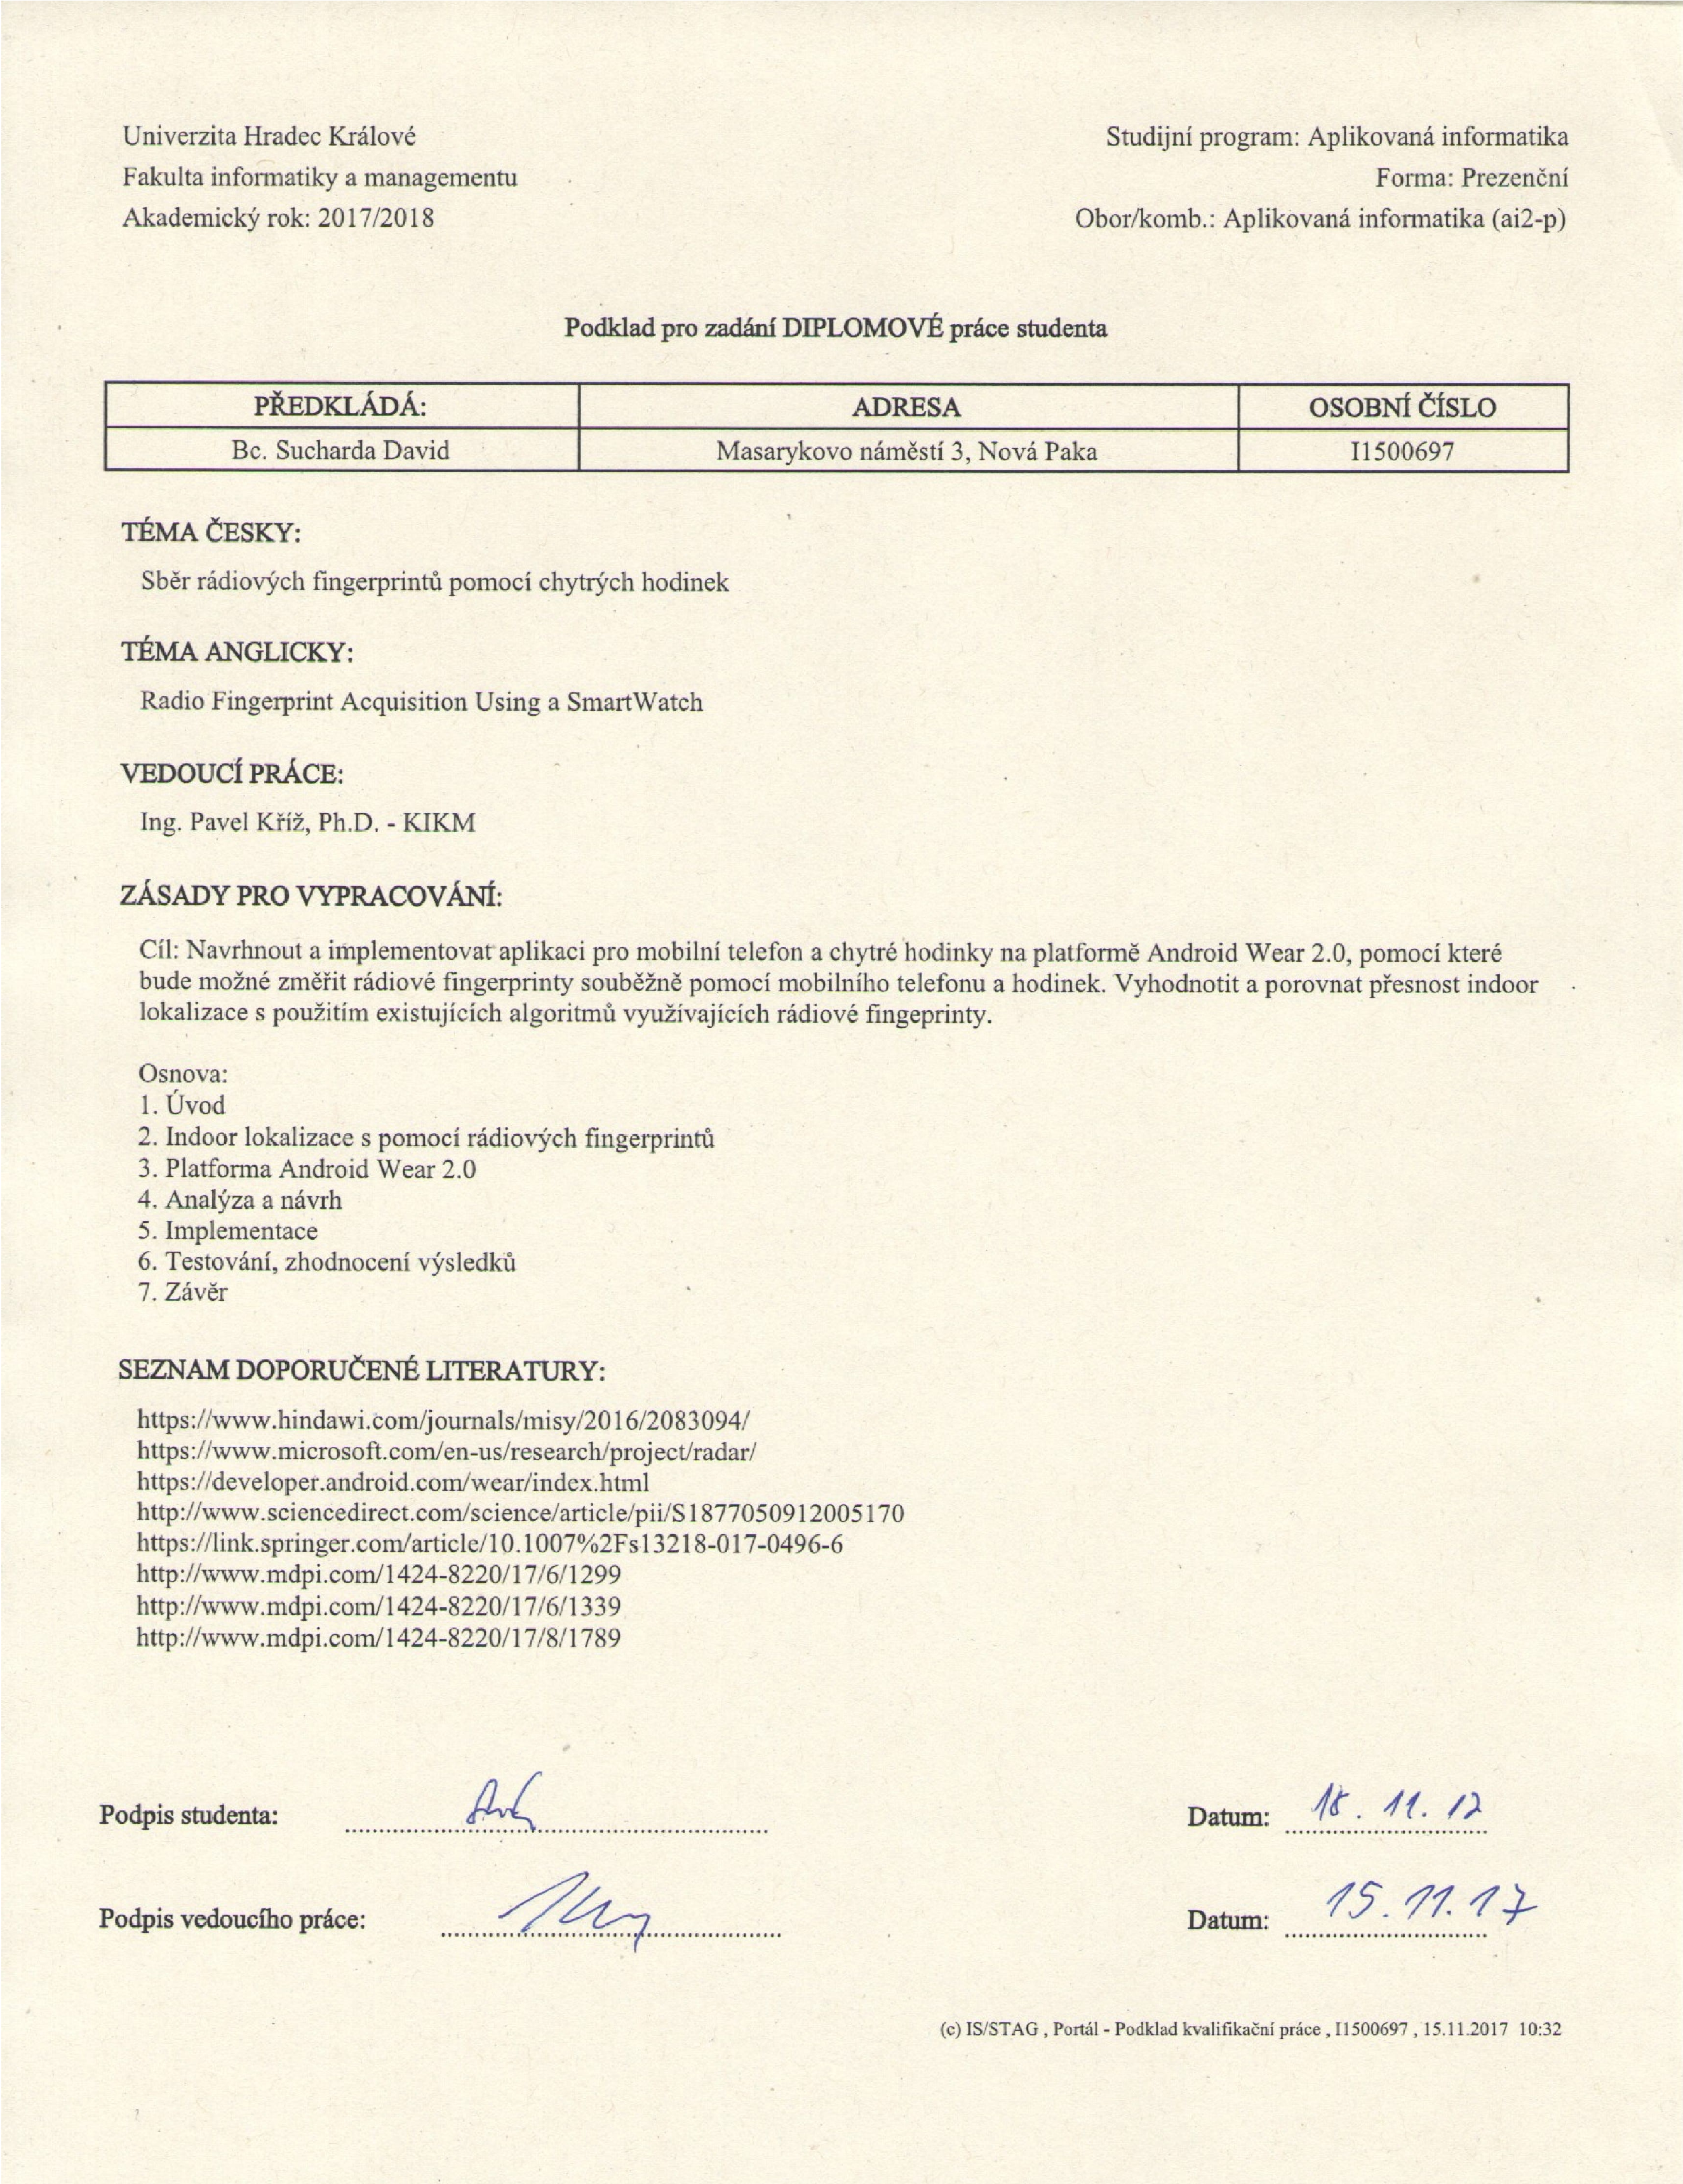
\includepdf[pages={1}]{assignment.pdf}

\end{document}